\documentclass[11pt,a4paper,oneside]{report}

\usepackage[utf8]{inputenc}
\usepackage[T1]{fontenc}
\usepackage[italian]{babel}
\usepackage{lmodern}
\usepackage{microtype}
\usepackage{graphicx}
\usepackage{caption}
\captionsetup{font={small,sf}, labelfont=bf}
\usepackage[top=2.5cm, bottom=2.5cm, left=2.5cm, right=2.5cm]{geometry}

\usepackage{amsmath,amssymb,amsthm,mathtools,bm}
\usepackage{booktabs}
\usepackage{tabularx}
\usepackage{array}
\usepackage{enumitem}
\usepackage{fancyhdr}
\usepackage{titlesec}
\usepackage{xcolor}
\usepackage{float}
\usepackage[most]{tcolorbox}
\usepackage{tikz}
\usetikzlibrary{shapes.geometric,calc,arrows.meta}

\usepackage[colorlinks=true,
            linkcolor=blue!80!black,
            citecolor=teal!80!black,
            urlcolor=cyan!80!black,
            bookmarksdepth=3]{hyperref}

% Palette cromatica ad alto contrasto (Standard Master 4.0 - Light Theme)
\definecolor{primaryBlue}{RGB}{24, 76, 120}
\definecolor{slateBg}{RGB}{248, 250, 252}
\definecolor{slateBorder}{RGB}{203, 213, 225}
\definecolor{accentGreen}{RGB}{22, 163, 74}
\definecolor{accentAmber}{RGB}{217, 119, 6}
\definecolor{accentRed}{RGB}{220, 38, 38}
\definecolor{accentPurple}{RGB}{124, 58, 237}
\definecolor{textDark}{RGB}{15, 23, 42}
\colorlet{amber}{accentAmber}

% Ambienti didattici rigorosi (Standard Master 4.0)
\newtcolorbox{definizione}[1][]{
  enhanced, breakable, colback=slateBg, colframe=primaryBlue,
  fonttitle=\bfseries\sffamily, title={Definizione e Teorema: #1},
  arc=3mm, boxrule=1pt, top=3mm, bottom=3mm, left=4mm, right=4mm
}

\newtcolorbox{aneddoto}[1][]{
  enhanced, breakable, colback=blue!4!white, colframe=primaryBlue,
  fonttitle=\bfseries\sffamily, title={Genesi Storica e Intuizione: #1},
  arc=3mm, boxrule=0.8pt, top=3mm, bottom=3mm, left=4mm, right=4mm
}

\newtcolorbox{laboratorio}[1][]{
  enhanced, breakable, colback=accentGreen!4!white, colframe=accentGreen,
  fonttitle=\bfseries\sffamily, title={Attivit\`a di Laboratorio Sperimentale: #1},
  arc=3mm, boxrule=0.8pt, top=3mm, bottom=3mm, left=4mm, right=4mm
}

\newtcolorbox{metodo}[1][]{
  enhanced, breakable, colback=accentAmber!4!white, colframe=accentAmber,
  fonttitle=\bfseries\sffamily, title={Metodo Operativo e Dimostrazione: #1},
  arc=3mm, boxrule=0.8pt, top=3mm, bottom=3mm, left=4mm, right=4mm
}

\pagestyle{fancy}
\fancyhf{}
\fancyhead[L]{\small\sffamily Liceo Scientifico Statale «Leonardo da Vinci» – Maglie}
\fancyhead[R]{\small\sffamily Lab. Matematico – Classe 1B}
\fancyfoot[C]{\thepage}
\renewcommand{\headrulewidth}{0.4pt}

\titleformat{\chapter}[display]
  {\normalfont\sffamily\huge\bfseries\color{primaryBlue}}
  {\chaptertitlename\ \thechapter}{15pt}{\Huge}

\begin{document}

% Frontespizio Formale Istituzionale
\hypersetup{pageanchor=false}
\begin{titlepage}
\begin{center}
  \vspace*{0.8cm}
  {\Large\textbf{LICEO SCIENTIFICO STATALE «LEONARDO DA VINCI»}}\\[0.25cm]
  {\large\textbf{MAGLIE (LE)}}\\[1.8cm]
  \rule{\textwidth}{1.5pt}\\[0.6cm]
  {\fontsize{24}{32}\selectfont\bfseries\color{primaryBlue} QUADERNO DI LABORATORIO\\[0.25cm] MATEMATICO\par}\vspace{0.5cm}
  {\fontsize{13}{19}\selectfont\bfseries\color{textDark} SOMMATORIE DI GAUSS, NUMERI FIGURATI PITAGORICI,\\[0.15cm] CRITERI DI DIVISIBILIT\`A ED APPROSSIMAZIONI DI $\pi$\par}\vspace{0.5cm}
  \rule{\textwidth}{1.5pt}\\[2.0cm]
  
  \begin{minipage}{0.48\textwidth}
    \textbf{Docente:}\\
    Prof. Giuseppe De Pascali\\
    \textit{Matematica e Fisica}
  \end{minipage}
  \hfill
  \begin{minipage}{0.48\textwidth}
    \raggedleft
    \textbf{Classe:}\\
    1\textordfeminine\ Sezione B\\
    \textit{Liceo Scientifico Tradizionale}\\
    Anno Scolastico 2026/2027
  \end{minipage}

  \vfill
  {\small Compendio Didattico Rigoroso ad Alto Contrasto (Standard Master 4.0 -- Tema Chiaro Perenne)}
\end{center}
\end{titlepage}
\hypersetup{pageanchor=true}
\pagenumbering{roman}

\tableofcontents
\newpage
\pagenumbering{arabic}

% ==============================================================================
% CAPITOLO 1
% ==============================================================================
\chapter{La Somma dei Primi \texorpdfstring{$n$}{n} Numeri Naturali e il Metodo di Gauss}

\section{L'Intuizione del Giovane Carl Friedrich Gauss}
\begin{aneddoto}[L'Episodio della Scuola Elementare di Braunschweig]
Nel 1787, all'et\`a di soli nove anni, Carl Friedrich Gauss lasci\`o sbigottito il maestro B\"uttner risolvendo in pochi istanti il compito punitivo assegnato alla classe: determinare la somma di tutti i numeri interi da $1$ a $100$:
\[
S = 1 + 2 + 3 + \dots + 98 + 99 + 100
\]
Anzich\'e eseguire 99 addizioni sequenziali faticose e soggette a errore, Gauss colse una simmetria strutturale profonda nel reticolo dei numeri:
\begin{itemize}[leftmargin=2em]
  \item Accoppiando il primo con l'ultimo termine: $1 + 100 = 101$;
  \item Accoppiando il secondo con il penultimo: $2 + 99 = 101$;
  \item Accoppiando il terzo con il terzultimo: $3 + 98 = 101$;
  \item Proseguendo sistematicamente fino al centro della sequenza: $50 + 51 = 101$.
\end{itemize}
Essendovi esattamente $50$ coppie distinte, ciascuna avente somma costante pari a $101$, il valore complessivo della sommatoria si ottiene tramite una singola moltiplicazione:
\[
S = 50 \cdot 101 = 5050
\]
Tale procedimento trasforma un calcolo computazionalmente oneroso di complessit\`a lineare in una procedura immediata a tempo costante.
\end{aneddoto}

\section{Dimostrazione Rigorosa della Formula di Gauss}
\begin{definizione}[Formula Chiusa per la Somma dei Primi $n$ Interi]
Per ogni intero positivo $n \in \mathbb{N}^+$, la somma dei primi $n$ numeri naturali consecutivi \`e espressa dalla formula chiusa:
\[
S_n = \sum_{k=1}^n k = 1 + 2 + 3 + \dots + n = \frac{n(n + 1)}{2}
\]
\end{definizione}

\noindent
\textbf{Dimostrazione per Ribaltamento della Somma (Metodo di Gauss):}\\
Consideriamo la somma $S_n$ scritta due volte, la prima in ordine strettamente crescente e la seconda in ordine strettamente decrescente:
\[
\begin{array}{rccccccccc}
S_n & = & 1 & + & 2 & + & 3 & + \dots + & n \\
S_n & = & n & + & (n-1) & + & (n-2) & + \dots + & 1 \\
\hline
2S_n & = & (n+1) & + & (n+1) & + & (n+1) & + \dots + & (n+1)
\end{array}
\]
Sommando membro a membro le due uguaglianze, ogni colonna $k$-esima fornisce come somma:
\[
k + (n - k + 1) = n + 1
\]
Poich\'e le colonne sono esattamente $n$, la somma a secondo membro \`e composta da $n$ addendi identici uguali a $(n + 1)$. Si ottiene pertanto l'equazione:
\[
2S_n = n(n + 1) \implies S_n = \frac{n(n + 1)}{2}
\]
La formula risulta cos\`i dimostrata in modo ineccepibile per qualsiasi intero naturale $n \ge 1$.

\section{Laboratorio Sperimentale: Somma di \texorpdfstring{$m$}{m} Numeri Consecutivi a Partire da \texorpdfstring{$n$}{n}}
\begin{laboratorio}[Indagine Sperimentale del Manoscritto (Tavola 1 e Tavola 7)]
Nel laboratorio di aritmetica sperimentale, consideriamo la somma $S(n, m)$ di $m$ numeri interi positivi consecutivi a partire da un generico intero $n$:
\[
S(n, m) = n + (n+1) + (n+2) + \dots + (n + m - 1)
\]
Raggruppando gli $m$ termini uguali a $n$ e applicando la formula di Gauss alla parte restante:
\[
S(n, m) = m \cdot n + \sum_{k=0}^{m-1} k = m \cdot n + \frac{(m-1)m}{2} = m \left( n + \frac{m-1}{2} \right)
\]
Analizziamo i casi concreti indagati sperimentalmente dagli studenti:
\begin{enumerate}[leftmargin=2em]
  \item \textbf{Caso $m = 2$ (Somma di 2 numeri consecutivi):}
  \[
  S(n, 2) = n + (n+1) = 2n + 1
  \]
  La somma di due interi consecutivi \`e \textbf{sempre un numero dispari}, poich\'e uno dei due addendi \`e necessariamente pari e l'altro \`e dispari.
  \item \textbf{Caso $m = 3$ (Somma di 3 numeri consecutivi -- Tavola 7):}
  \[
  S(n, 3) = n + (n+1) + (n+2) = 3n + 3 = 3(n+1)
  \]
  La somma di tre interi consecutivi \`e \textbf{sempre divisibile per 3}, ed \`e esattamente uguale al triplo del termine centrale $(n+1)$.\\
  \textbf{Condizione di divisibilit\`a per 7:} Poich\'e $S(n, 3) = 3(n+1)$ e $\mathrm{MCD}(3, 7) = 1$, per il lemma di Euclide si ha:
  \[
  7 \mid S(n, 3) \iff 7 \mid (n+1) \iff n \equiv 6 \pmod 7
  \]
  I valori di $n$ che generano una somma divisibile per 7 formano una progressione aritmetica di ragione 7:
  \[
  n \in \{6, 13, 20, 27, 34, \dots\}
  \]
  \textit{Verifiche sperimentali del quaderno:}
  \begin{itemize}
    \item $n = 6 \implies 6 + 7 + 8 = 21 = 3 \cdot 7$ (divisibile per 7);
    \item $n = 13 \implies 13 + 14 + 15 = 42 = 6 \cdot 7$ (divisibile per 7);
    \item $n = 20 \implies 20 + 21 + 22 = 63 = 9 \cdot 7$ (divisibile per 7).
  \end{itemize}
  \item \textbf{Caso $m = 4$ (Somma di 4 numeri consecutivi -- Tavola 1):}
  \[
  S(n, 4) = n + (n+1) + (n+2) + (n+3) = 4n + 6 = 2(2n + 3)
  \]
  Tale somma \`e sempre pari ma \textbf{mai multipla di 4}. Per $n = 2$ si ottiene:
  \[
  S(2, 4) = 2 + 3 + 4 + 5 = 14 \quad (\text{divisibile per } 7)
  \]
  \item \textbf{Caso $m = 7$ (Somma di 7 numeri consecutivi -- Tavola 1):}
  \[
  S(n, 7) = 7n + \frac{6 \cdot 7}{2} = 7n + 21 = 7(n + 3)
  \]
  La somma di 7 numeri interi consecutivi \`e \textbf{SEMPRE divisibile per 7}, per qualunque valore di $n \in \mathbb{N}$!\\
  \textit{Verifiche del manoscritto:}
  \begin{itemize}
    \item $n = 2 \implies 2+3+4+5+6+7+8 = 35 = 5 \cdot 7$;
    \item $n = 3 \implies 3+4+5+6+7+8+9 = 42 = 6 \cdot 7$;
    \item $n = 4 \implies 4+5+6+7+8+9+10 = 49 = 7 \cdot 7$.
  \end{itemize}
\end{enumerate}
\end{laboratorio}

% ==============================================================================
% CAPITOLO 2
% ==============================================================================
\chapter{Geometria Aritmetica: I Numeri Figurati}

\section{Genesi Pitagorica e Accompagnamento Visuale}
Nella scuola pitagorica (VI sec. a.C.), il numero non era concepito come una mera entit\`a simbolica astratta, bens\`i come una configurazione geometrica discreta formata da sassolini (\textit{calculi}) disposti nello spazio secondo precise simmetrie poligonali regolari.
In ossequio al principio didattico per cui \textbf{le figure devono sempre accompagnare i concetti}, ogni classe di numeri figurati viene qui introdotta affiancando alla trattazione analitica la sua rigorosa rappresentazione grafica TikZ a reticolo puntiforme, priva di sovrapposizioni.

\section{Numeri Triangolari (\texorpdfstring{$T_n$}{Tn})}
\begin{definizione}[Numero Triangolare]
Un numero naturale $T_n$ si definisce \textbf{triangolare} se pu\`o essere geometricamente disposto sotto forma di triangolo equilatero discreto a reticolo regolare.
La relazione di ricorrenza fondamentale esprime l'aggiunta di una nuova riga basale di $(n+1)$ elementi al triangolo di ordine $n$:
\[
T_{n+1} = T_n + (n+1), \quad \text{con } T_1 = 1
\]
La formula esplicita chiusa coincide con la sommatoria di Gauss:
\[
T_n = \sum_{k=1}^n k = \frac{n(n+1)}{2}
\]
I primi termini della successione sono:
\[
T_1 = 1, \quad T_2 = 3, \quad T_3 = 6, \quad T_4 = 10, \quad T_5 = 15, \quad T_6 = 21, \quad T_7 = 28
\]
\end{definizione}

\begin{figure}[H]
\centering
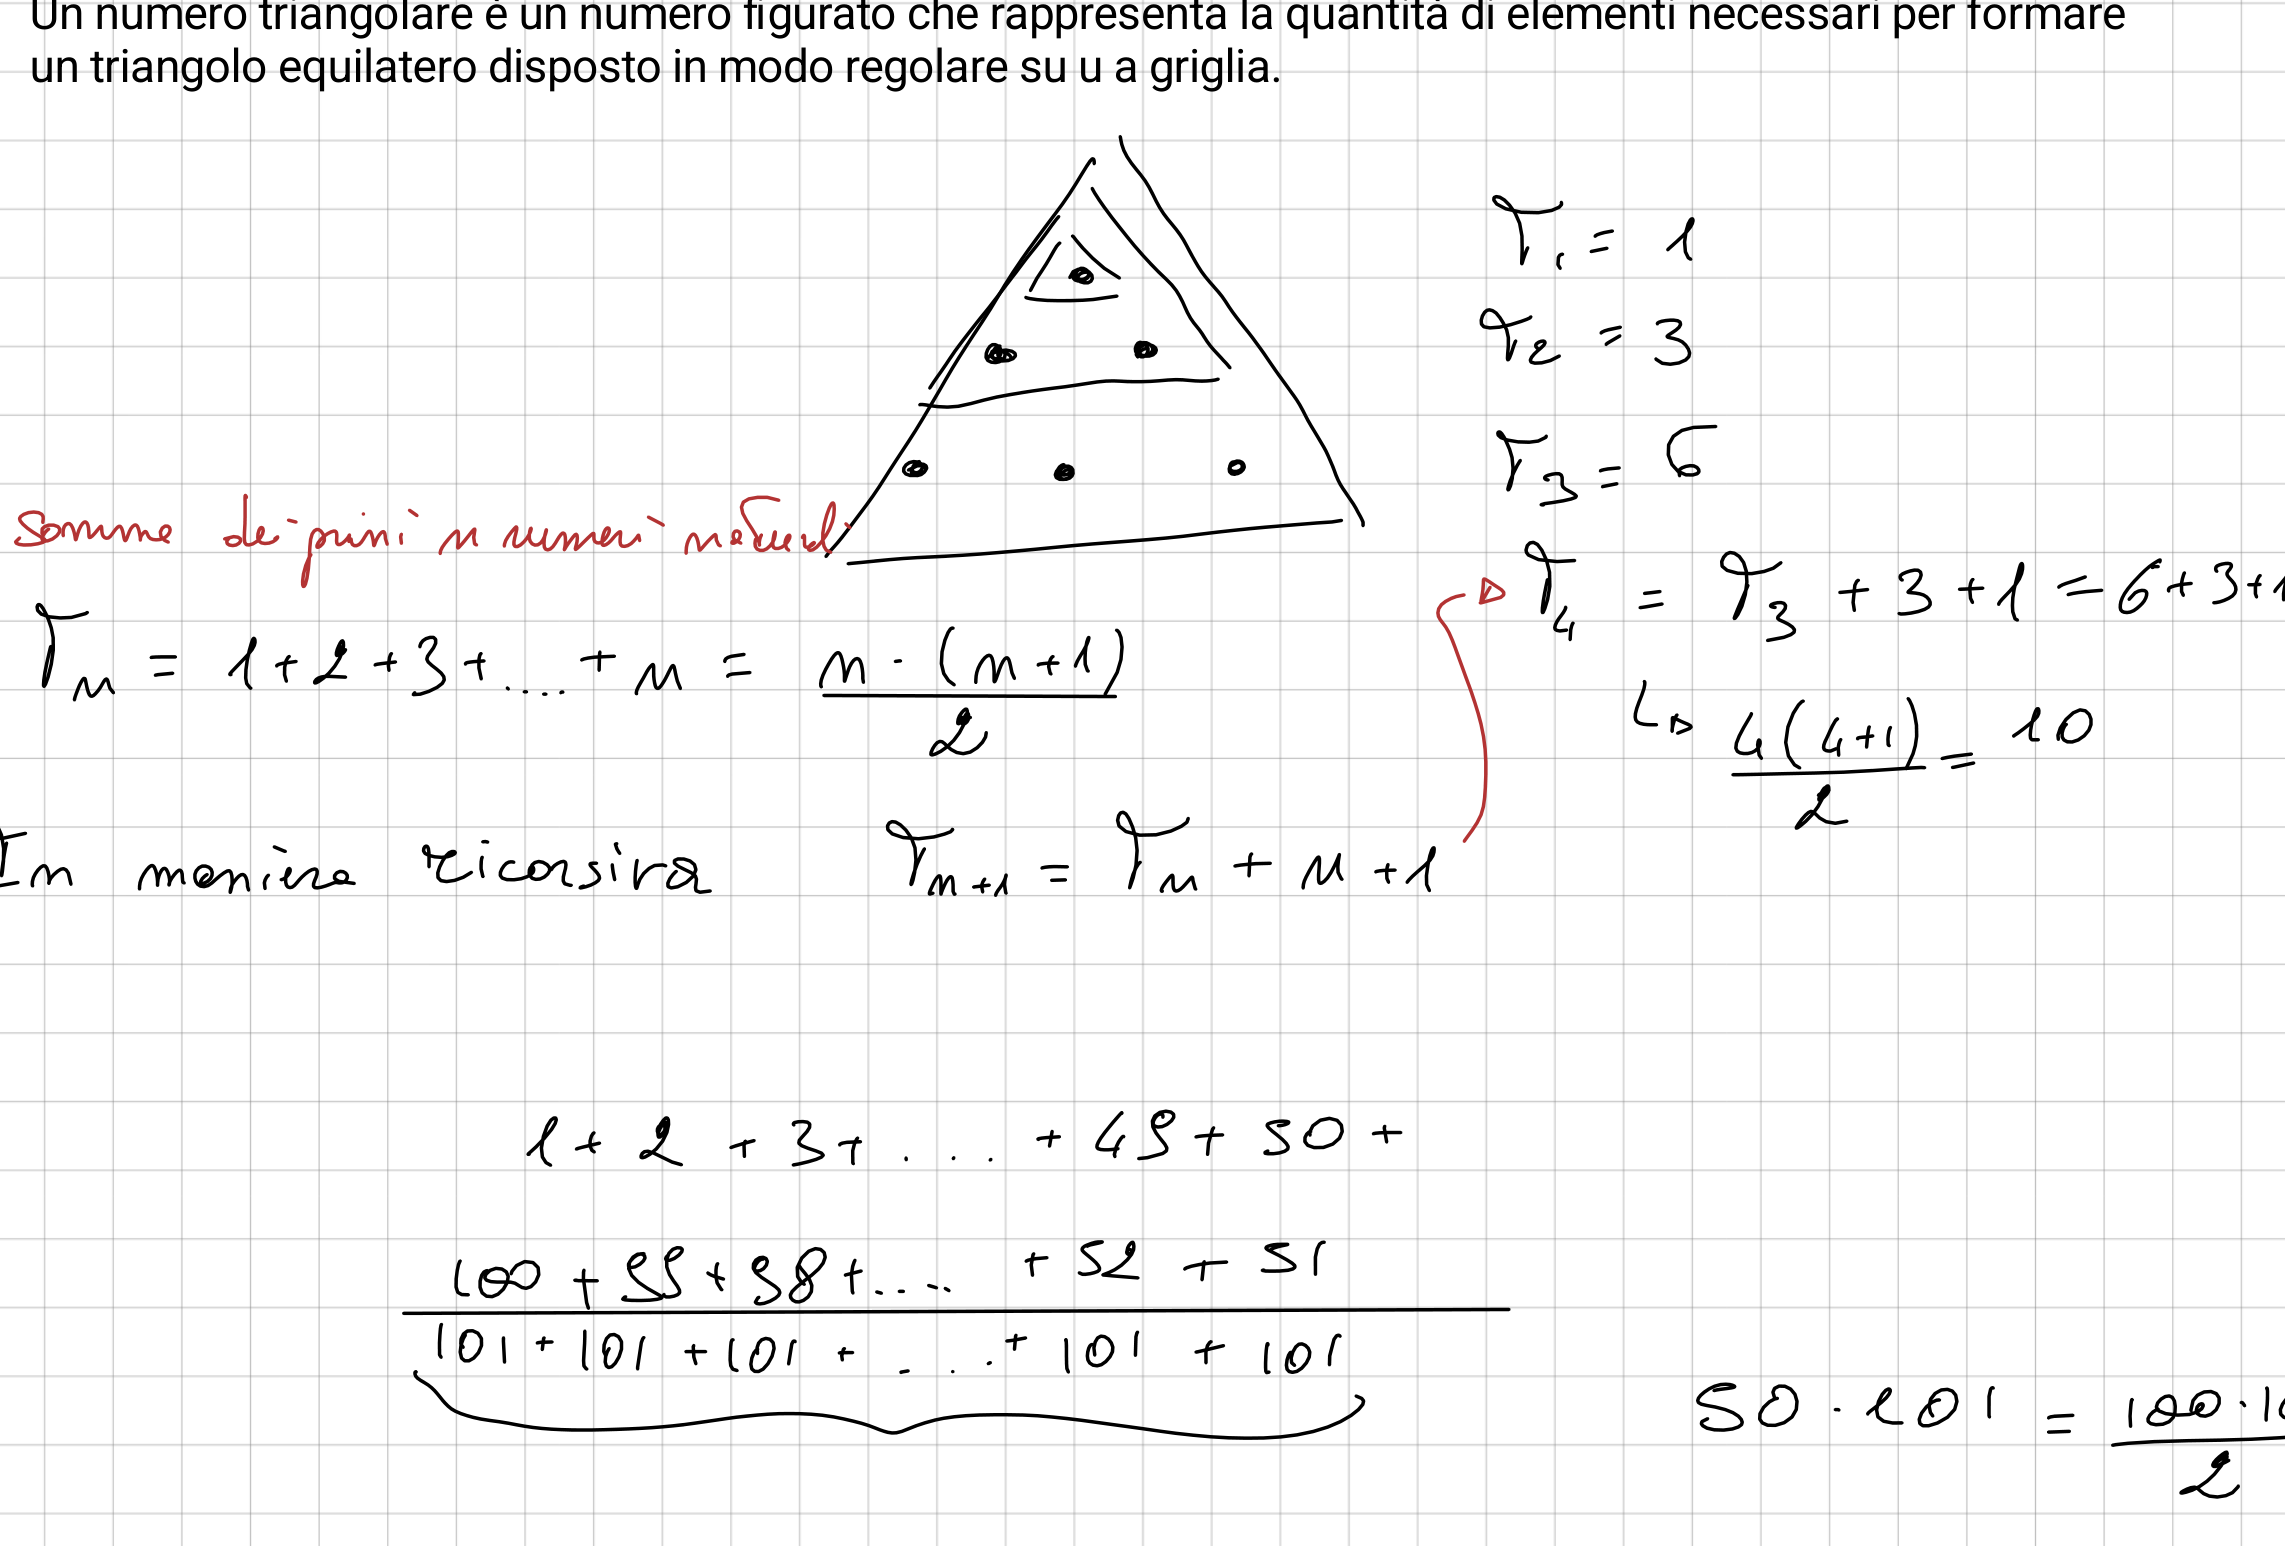
\includegraphics[width=0.88\linewidth]{immagini/appunti_triangolari_gauss.png}
\caption{Riproduzione fedele della Tavola 2 originale: triangolo a strati orizzontali $T_1=1, T_2=3, T_3=6, T_4=10$, formula ricorsiva $T_{n+1} = T_n + n + 1$ e dimostrazione di Gauss per coppie da 101.}
\end{figure}

\begin{figure}[H]
\centering
\begin{tikzpicture}[scale=0.68]
  % T_1 = 1
  \begin{scope}[xshift=0cm]
    \node at (0, 3.4) {\textbf{\color{primaryBlue}$T_1 = 1$}};
    \fill[primaryBlue] (0, 1.2) circle (4.5pt);
    \node[below, font=\scriptsize, text=gray!80!black] at (0, 0.4) {$n=1$};
  \end{scope}

  % T_2 = 3
  \begin{scope}[xshift=3.2cm]
    \node at (0.5, 3.4) {\textbf{\color{primaryBlue}$T_2 = 3$}};
    \fill[primaryBlue] (0.5, 1.8) circle (4.5pt);
    \fill[primaryBlue] (0, 0.934) circle (4.5pt);
    \fill[primaryBlue] (1.0, 0.934) circle (4.5pt);
    \draw[thick, primaryBlue!40] (0.5, 1.8) -- (0, 0.934) -- (1.0, 0.934) -- cycle;
    \node[below, font=\scriptsize, text=gray!80!black] at (0.5, 0.4) {$n=2$};
  \end{scope}

  % T_3 = 6
  \begin{scope}[xshift=7.2cm]
    \node at (1.0, 3.4) {\textbf{\color{primaryBlue}$T_3 = 6$}};
    \fill[primaryBlue] (1.0, 2.4) circle (4.5pt);
    \fill[primaryBlue] (0.5, 1.534) circle (4.5pt);
    \fill[primaryBlue] (1.5, 1.534) circle (4.5pt);
    \fill[primaryBlue] (0, 0.668) circle (4.5pt);
    \fill[primaryBlue] (1.0, 0.668) circle (4.5pt);
    \fill[primaryBlue] (2.0, 0.668) circle (4.5pt);
    \draw[thick, primaryBlue!40] (1.0, 2.4) -- (0, 0.668) -- (2.0, 0.668) -- cycle;
    \node[below, font=\scriptsize, text=gray!80!black] at (1.0, 0.2) {$n=3$};
  \end{scope}

  % T_4 = 10
  \begin{scope}[xshift=12.2cm]
    \node at (1.5, 3.4) {\textbf{\color{primaryBlue}$T_4 = 10$}};
    \fill[primaryBlue] (1.5, 3.0) circle (4.5pt);
    \fill[primaryBlue] (1.0, 2.134) circle (4.5pt);
    \fill[primaryBlue] (2.0, 2.134) circle (4.5pt);
    \fill[primaryBlue] (0.5, 1.268) circle (4.5pt);
    \fill[primaryBlue] (1.5, 1.268) circle (4.5pt);
    \fill[primaryBlue] (2.5, 1.268) circle (4.5pt);
    \fill[primaryBlue] (0, 0.402) circle (4.5pt);
    \fill[primaryBlue] (1.0, 0.402) circle (4.5pt);
    \fill[primaryBlue] (2.0, 0.402) circle (4.5pt);
    \fill[primaryBlue] (3.0, 0.402) circle (4.5pt);
    \draw[thick, primaryBlue!40] (1.5, 3.0) -- (0, 0.402) -- (3.0, 0.402) -- cycle;
    \node[below, font=\scriptsize, text=gray!80!black] at (1.5, 0.0) {$n=4$};
  \end{scope}
\end{tikzpicture}
\caption{Rappresentazione a reticolo triangolare equilatero dei primi 4 numeri triangolari ($T_1=1, T_2=3, T_3=6, T_4=10$).}
\end{figure}

\section{Numeri Quadrati (\texorpdfstring{$Q_n$}{Qn}) e la Somma dei Primi \texorpdfstring{$n$}{n} Dispari}
\begin{definizione}[Numero Quadrato e Teorema dello Gnomone]
Un numero naturale $Q_n$ si definisce \textbf{quadrato perfetto} se corrisponde agli elementi di una matrice quadrata regolare di lato $n$:
\[
Q_n = n^2
\]
La relazione di ricorrenza esprime la crescita da un quadrato di lato $(n-1)$ al successivo tramite l'aggiunta di una squadra di punti (\textit{gnomone}) sui due lati esterni:
\[
Q_n = Q_{n-1} + (2n - 1), \quad \text{con } Q_1 = 1
\]
Ne discende il fondamentale \textbf{Teorema dello Gnomone Pitagorico}: la somma dei primi $n$ numeri naturali dispari \`e sempre un quadrato perfetto:
\[
Q_n = \sum_{k=1}^n (2k - 1) = 1 + 3 + 5 + \dots + (2n - 1) = n^2
\]
\end{definizione}

\noindent
\textbf{Verifica dal Manoscritto (Tavola 2 e Tavola 3):}
\begin{itemize}[leftmargin=2em]
  \item $Q_1 = 1^2 = 1$;
  \item $Q_2 = 1 + 3 = 4 = 2^2$;
  \item $Q_3 = 1 + 3 + 5 = 9 = 3^2$;
  \item $Q_4 = 1 + 3 + 5 + 7 = 16 = 4^2$;
  \item $Q_9 = 1 + 3 + 5 + \dots + 17 = 81 = 9^2$;
  \item $Q_{10} = Q_9 + (2 \cdot 10 - 1) = 81 + 19 = 100 = 10^2$.
\end{itemize}

\begin{figure}[H]
\centering
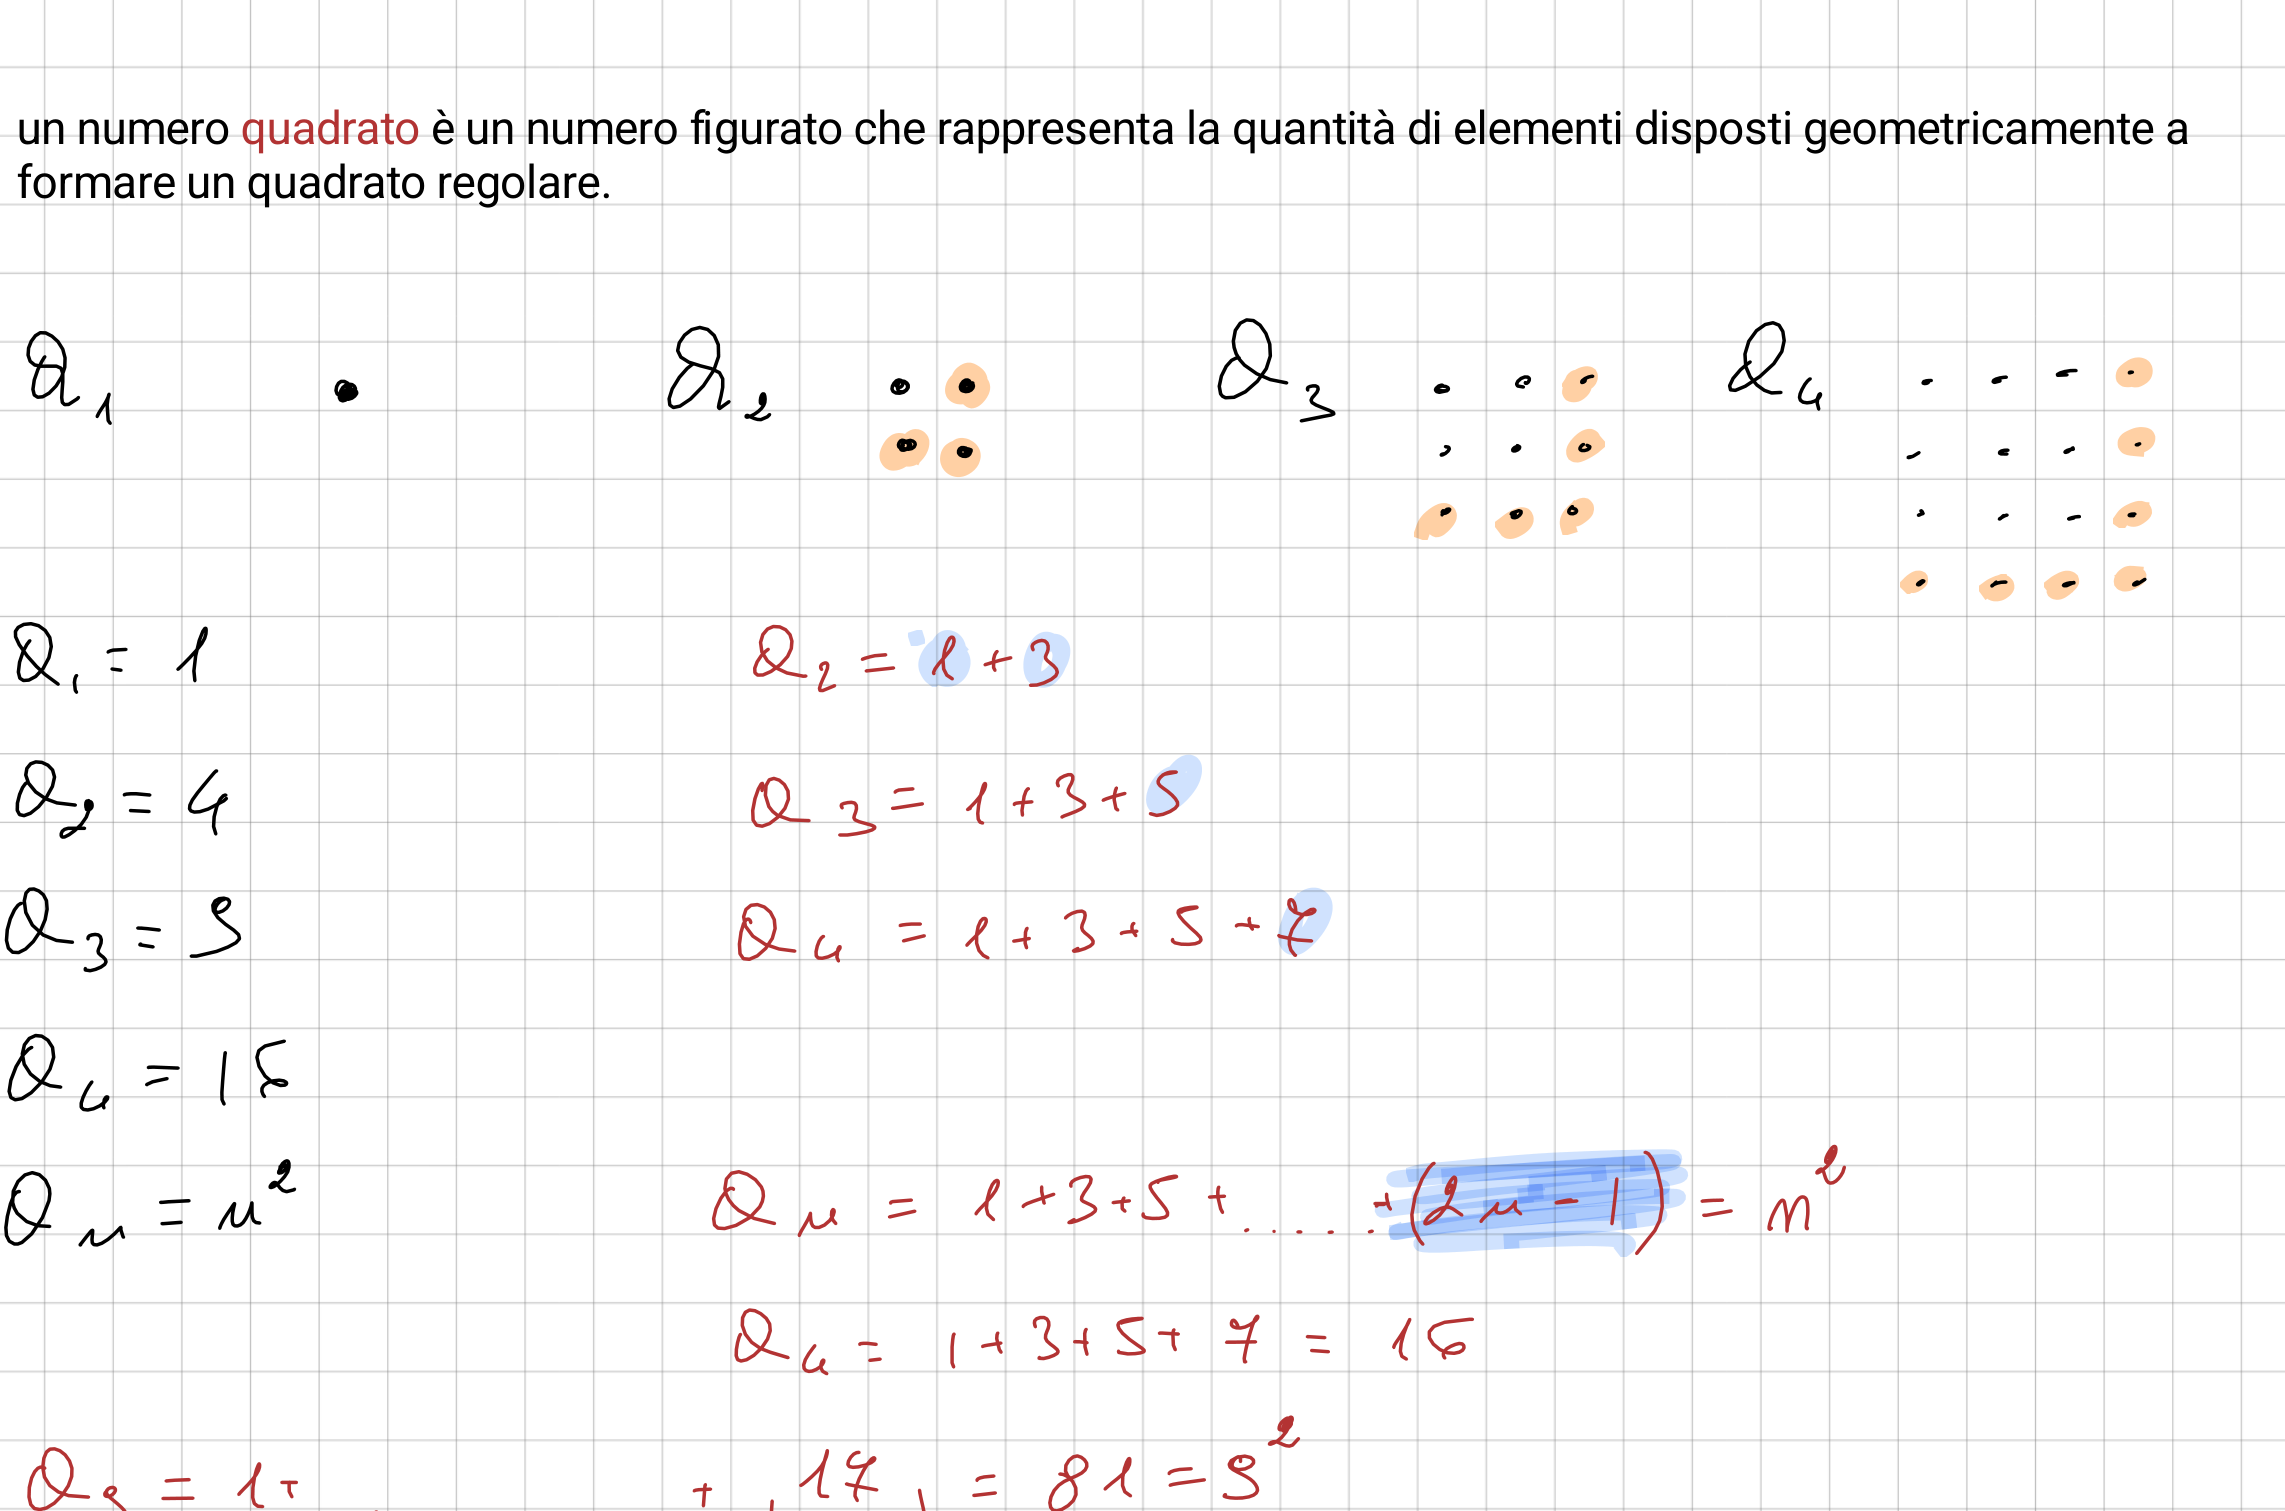
\includegraphics[width=0.88\linewidth]{immagini/appunti_quadrati_gnomone.png}
\caption{Riproduzione fedele della Tavola 2 originale: numeri quadrati $Q_1, Q_2, Q_3, Q_4$ con gnomoni e somma dei primi $n$ numeri dispari.}
\end{figure}

\begin{figure}[H]
\centering
\begin{tikzpicture}[scale=0.7]
  % Q_1 = 1
  \begin{scope}[xshift=0cm]
    \node at (0, 3.5) {\textbf{\color{accentGreen}$Q_1 = 1$}};
    \fill[accentGreen] (0, 1.5) circle (4.5pt);
  \end{scope}

  % Q_2 = 4
  \begin{scope}[xshift=2.6cm]
    \node at (0.5, 3.5) {\textbf{\color{accentGreen}$Q_2 = 4$}};
    \foreach \r in {0,1} {
      \foreach \c in {0,1} {
        \fill[accentGreen] (\c, \r+1.0) circle (4.5pt);
      }
    }
  \end{scope}

  % Q_3 = 9
  \begin{scope}[xshift=6.0cm]
    \node at (1.0, 3.5) {\textbf{\color{accentGreen}$Q_3 = 9$}};
    \foreach \r in {0,1,2} {
      \foreach \c in {0,1,2} {
        \fill[accentGreen] (\c, \r+0.5) circle (4.5pt);
      }
    }
  \end{scope}

  % Q_4 = 16 Gnomonico
  \begin{scope}[xshift=10.6cm]
    \node at (1.5, 3.5) {\textbf{\color{accentGreen}$Q_4 = 16$ (Gnomoni)}};
    % Gnomone 1 (blu) k=1: 1 punto
    \fill[primaryBlue] (0, 3) circle (4.5pt);
    
    % Gnomone 2 (verde) k=2: 3 punti
    \fill[accentGreen] (1, 3) circle (4.5pt);
    \fill[accentGreen] (1, 2) circle (4.5pt);
    \fill[accentGreen] (0, 2) circle (4.5pt);
    
    % Gnomone 3 (ambra) k=3: 5 punti
    \fill[accentAmber] (2, 3) circle (4.5pt);
    \fill[accentAmber] (2, 2) circle (4.5pt);
    \fill[accentAmber] (2, 1) circle (4.5pt);
    \fill[accentAmber] (1, 1) circle (4.5pt);
    \fill[accentAmber] (0, 1) circle (4.5pt);
    
    % Gnomone 4 (rosso) k=4: 7 punti
    \fill[accentRed] (3, 3) circle (4.5pt);
    \fill[accentRed] (3, 2) circle (4.5pt);
    \fill[accentRed] (3, 1) circle (4.5pt);
    \fill[accentRed] (3, 0) circle (4.5pt);
    \fill[accentRed] (2, 0) circle (4.5pt);
    \fill[accentRed] (1, 0) circle (4.5pt);
    \fill[accentRed] (0, 0) circle (4.5pt);

    \draw[thick, gray!50] (-0.3, 3.3) rectangle (0.3, 2.7);
    \draw[thick, gray!50] (-0.3, 3.3) rectangle (1.3, 1.7);
    \draw[thick, gray!50] (-0.3, 3.3) rectangle (2.3, 0.7);
    \draw[thick, gray!50] (-0.3, 3.3) rectangle (3.3, -0.3);
  \end{scope}
\end{tikzpicture}
\caption{Configurazioni dei numeri quadrati e decomposizione gnomonica a squadre concentriche di $Q_4 = 1 + 3 + 5 + 7 = 16$.}
\end{figure}

\section{Decomposizione Geometrica: \texorpdfstring{$Q_n = T_{n-1} + T_n$}{Qn = T{n-1} + Tn}}
\begin{metodo}[Teorema di Ricombinazione Pitagorica (Tavola 3 del Manoscritto)]
Ogni numero quadrato $Q_n$ si scompone naturalmente, lungo la diagonale principale del suo reticolo, nella somma di due numeri triangolari consecutivi:
\[
Q_n = T_n + T_{n-1}
\]
\textbf{Dimostrazione Algebrica Rigorosa:}
\[
T_n + T_{n-1} = \frac{n(n+1)}{2} + \frac{(n-1)n}{2} = \frac{n \big( (n+1) + (n-1) \big)}{2} = \frac{n(2n)}{2} = n^2 = Q_n
\]
Nel manoscritto, gli studenti hanno analizzato graficamente il caso per $n = 7$:
\[
Q_7 = 7^2 = 49 = T_7 + T_6 = 28 + 21
\]
\end{metodo}

\begin{figure}[H]
\centering
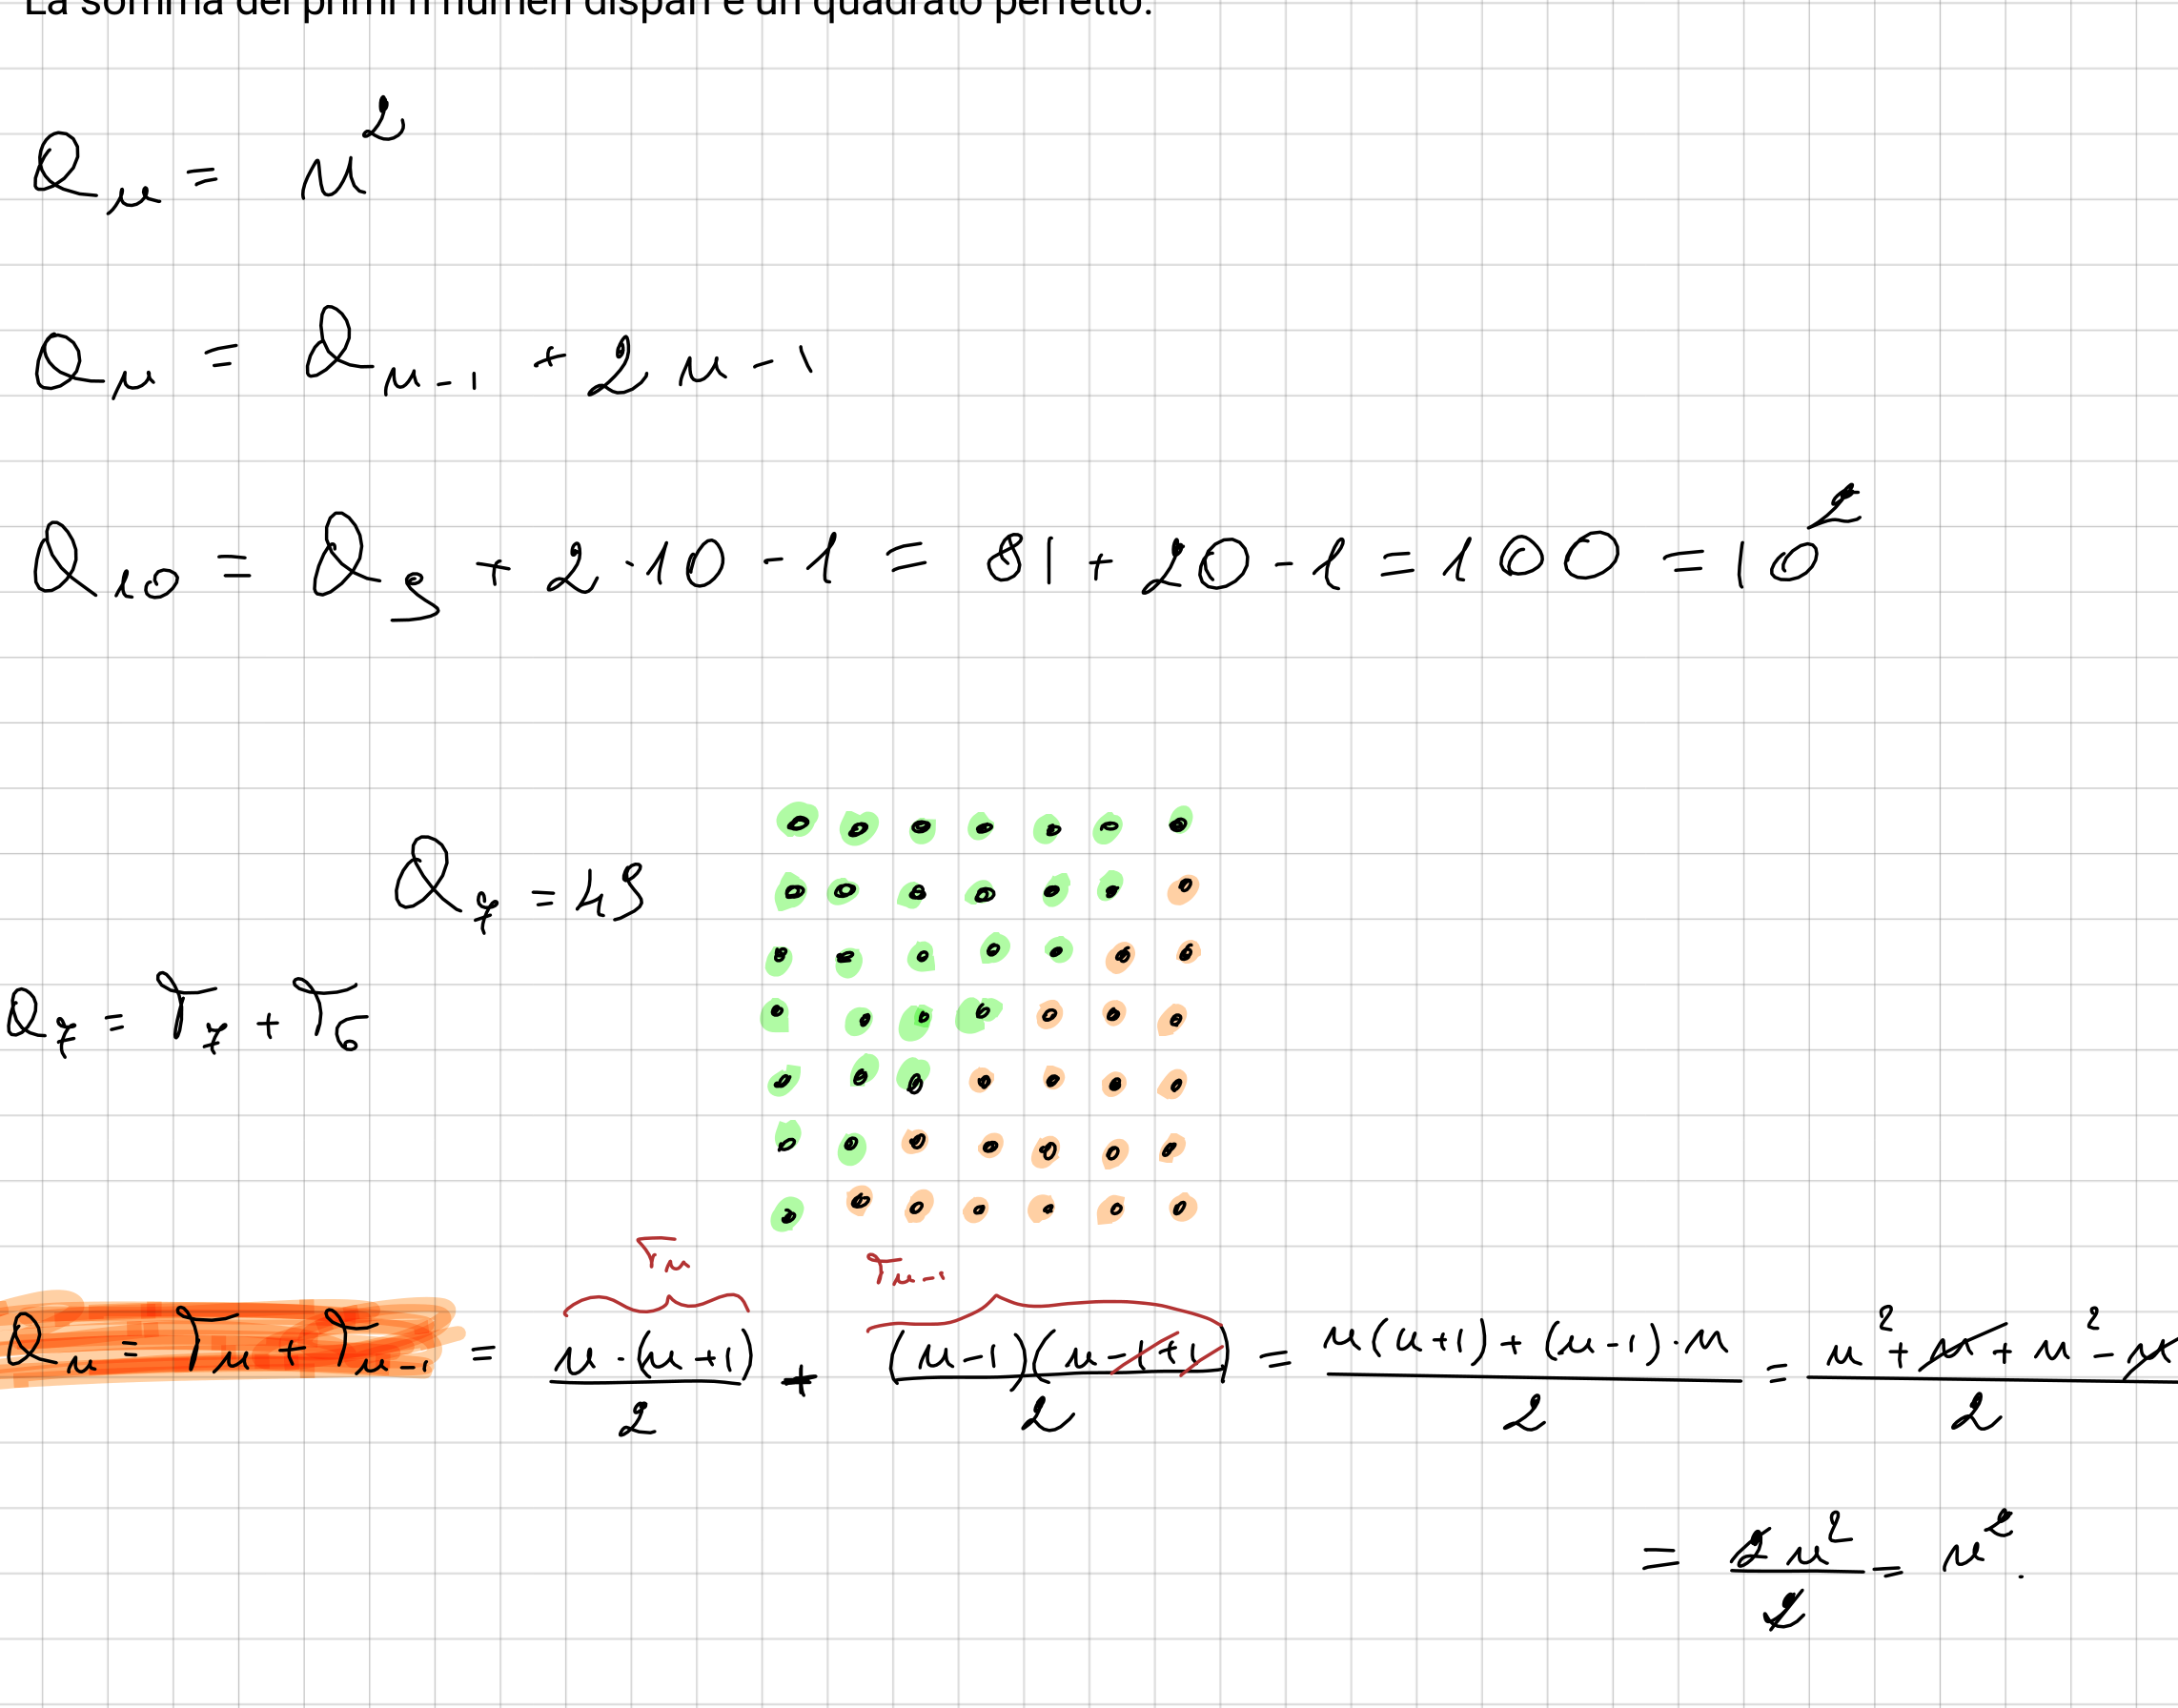
\includegraphics[width=0.88\linewidth]{immagini/appunti_q7_decomposizione.png}
\caption{Riproduzione fedele della Tavola 3 originale: reticolo $7\times 7$ con 28 punti verdi ($T_7$) e 21 punti arancioni ($T_6$) e dimostrazione $Q_n = T_n + T_{n-1} = n^2$.}
\end{figure}

\begin{figure}[H]
\centering
\begin{tikzpicture}[scale=0.6]
  \node at (3.0, 7.5) {\large\textbf{Decomposizione di $Q_7 = 49 = T_7 + T_6 = 28 + 21$}};
  
  % Griglia 7x7
  \foreach \r in {0,...,6} {
    \foreach \c in {0,...,6} {
      \pgfmathtruncatemacro{\cond}{\c <= \r ? 1 : 0}
      \ifnum\cond=1
        \fill[primaryBlue] (\c, \r) circle (4.5pt);
      \else
        \fill[accentAmber] (\c, \r) circle (4.5pt);
      \fi
    }
  }
  
  % Retta divisoria diagonale
  \draw[dashed, ultra thick, gray!80] (-0.4, -0.4) -- (6.4, 6.4);
  
  % Legenda compatta e centrata priva di collisioni
  \node[primaryBlue, font=\small\bfseries] at (3.0, -1.0) {$\bm{T_7 = 28}$ punti (blu: diagonale e triangolo inferiore)};
  \node[accentAmber, font=\small\bfseries] at (3.0, -1.6) {$\bm{T_6 = 21}$ punti (ambra: triangolo complementare superiore)};
  \node[font=\small] at (3.0, -2.2) {Somma totale reticolo: $28 + 21 = 49 = 7^2 = Q_7$};
\end{tikzpicture}
\caption{Dimostrazione visiva della scomposizione di $Q_7$ in due triangolari consecutivi $T_7$ e $T_6$ (conforme alla Tavola 3).}
\end{figure}

\section{Numeri Pentagonali (\texorpdfstring{$P_n$}{Pn})}
\begin{definizione}[Numero Pentagonale]
Un numero naturale $P_n$ si definisce \textbf{pentagonale} se rappresenta la quantit\`a di elementi necessari a formare geometricamente una sequenza di pentagoni regolari concentrici che condividono un vertice fisso comune.
I primi cinque termini della successione calcolati nel manoscritto sono:
\[
P_1 = 1, \quad P_2 = 5, \quad P_3 = 12, \quad P_4 = 22, \quad P_5 = 35
\]
\end{definizione}

\begin{figure}[H]
\centering
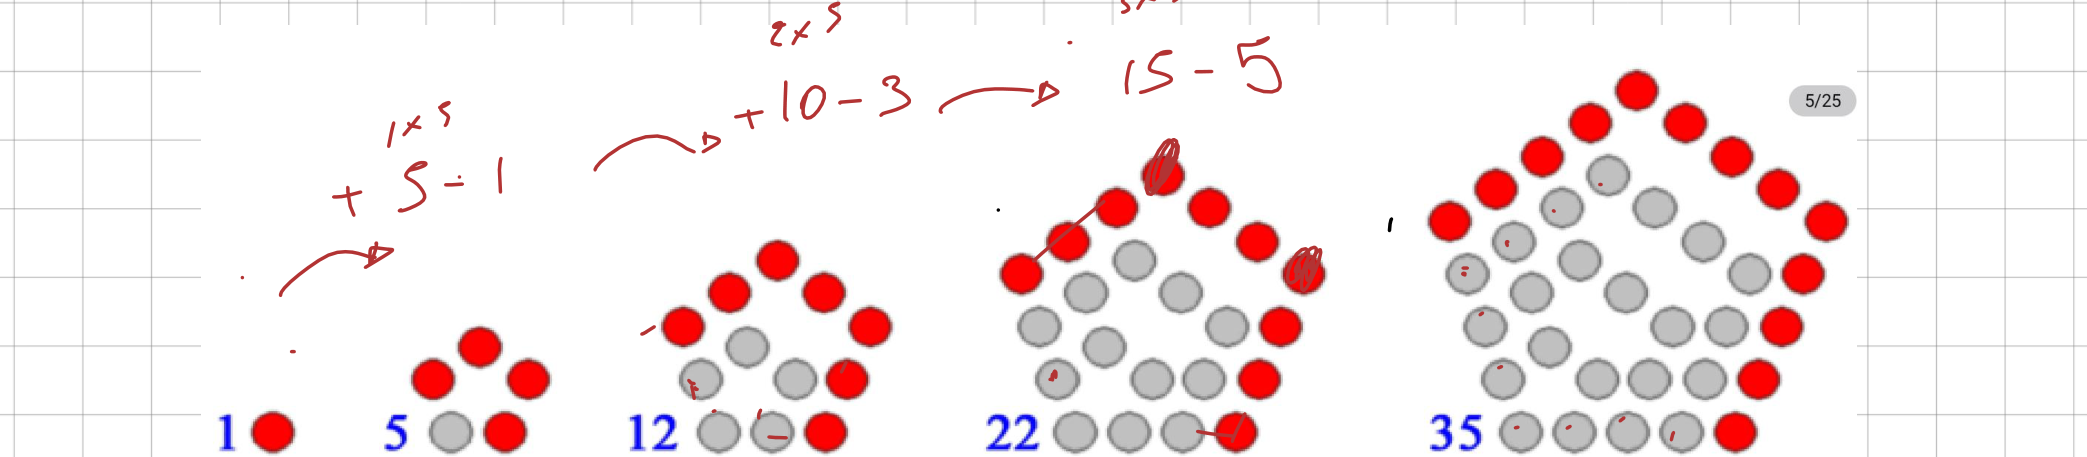
\includegraphics[width=0.88\linewidth]{immagini/traccia_numeri_pentagonali_libro.png}
\caption{Riproduzione fedele della diapositiva del libro di testo: configurazione geometrica dei primi cinque numeri pentagonali ($1, 5, 12, 22, 35$) con punti interni grigi e perimetro esterno rosso.}
\end{figure}

\begin{figure}[H]
\centering
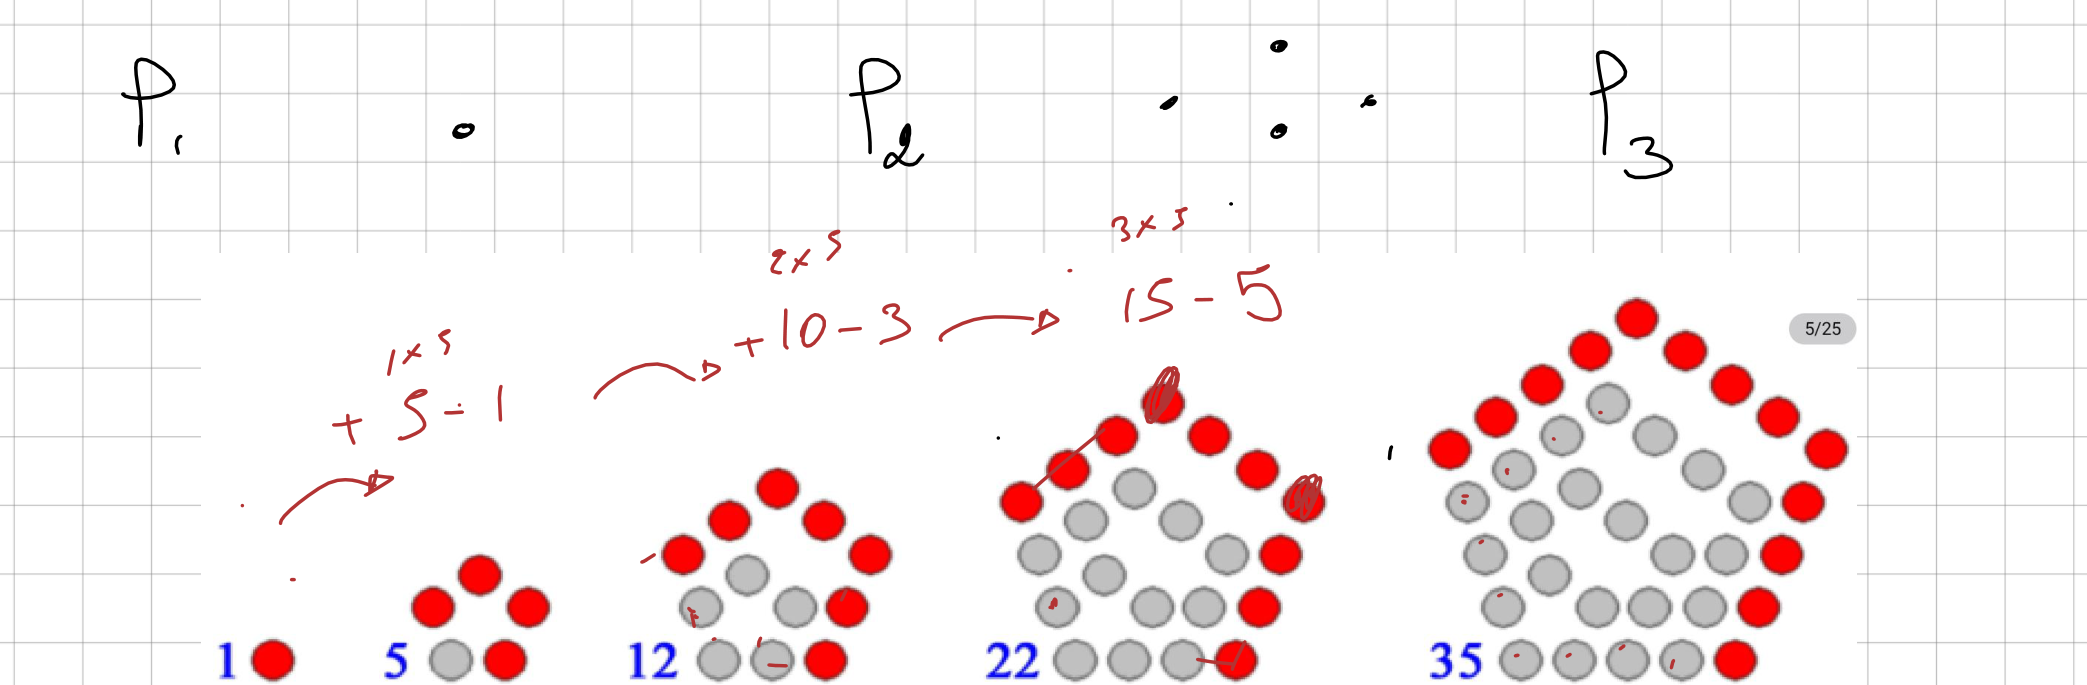
\includegraphics[width=0.88\linewidth]{immagini/traccia_numeri_pentagonali_annotata.png}
\caption{Riproduzione fedele degli appunti manoscritti (Tavola 3): incrementi per strati $+5-1$, $+10-3$, $+15-5$, legge ricorsiva $P_n = P_{n-1} + 3n - 2$ e formula chiusa.}
\end{figure}

\begin{metodo}[Genesi Ricorsiva e Dimostrazione Analitica del Manoscritto (Tavola 4)]
\textbf{1. Legge di Ricorrenza per Aggiunta di Lati:}\\
Dall'analisi degli strati concentrici del reticolo, ogni pentagono si ottiene dal precedente aggiungendo punti lungo 3 lati liberi:
\begin{align*}
P_1 &= 1 \\
P_2 &= P_1 + 4 = 5 \\
P_3 &= P_2 + 4 + 3 = 12 \\
P_4 &= P_3 + 4 + 3 + 3 = 22 \\
P_n &= P_{n-1} + 3n - 2
\end{align*}

\textbf{2. Dimostrazione Rigorosa della Formula Chiusa (Tavola 4 del Docente):}\\
Il docente esprime la somma degli incrementi successivi sottraendo le sovrapposizioni dei vertici in comune:
\[
1 + \underbrace{(5 - 1)}_{n=2} + \underbrace{(10 - 3)}_{n=3} + \underbrace{(15 - 5)}_{n=4} + \dots + \Big( 5(k-1) - (2k - 3) \Big)
\]
Sommando i contributi dei 5 lati per tutti i livelli ed eliminando i punti conteggiati pi\`u volte:
\[
P_n = 1 + 5 \sum_{k=1}^{n-1} k - (n - 1)^2
\]
Applicando la sommatoria di Gauss per $\sum_{k=1}^{n-1} k = \frac{n(n-1)}{2}$:
\[
P_n = 1 + \frac{5n(n-1)}{2} - (n^2 - 2n + 1)
\]
Riducendo a denominatore comune:
\[
P_n = \frac{5n^2 - 5n - 2(n^2 - 2n + 1) + 2}{2} = \frac{5n^2 - 5n - 2n^2 + 4n - 2 + 2}{2}
\]
Semplificando i termini opposti $-2 + 2 = 0$:
\[
P_n = \frac{3n^2 - n}{2} = \frac{n(3n - 1)}{2}
\]

\textbf{3. Verifica Termine a Termine:}
\begin{itemize}[leftmargin=2em]
  \item $P_1 = \dfrac{1(3 \cdot 1 - 1)}{2} = \dfrac{1 \cdot 2}{2} = 1$;
  \item $P_2 = \dfrac{2(3 \cdot 2 - 1)}{2} = \dfrac{2 \cdot 5}{2} = 5$;
  \item $P_3 = \dfrac{3(3 \cdot 3 - 1)}{2} = \dfrac{3 \cdot 8}{2} = 12$;
  \item $P_4 = \dfrac{4(3 \cdot 4 - 1)}{2} = \dfrac{4 \cdot 11}{2} = 22$;
  \item $P_5 = \dfrac{5(3 \cdot 5 - 1)}{2} = \dfrac{5 \cdot 14}{2} = 35$.
\end{itemize}
\end{metodo}

\begin{figure}[H]
\centering
\begin{tikzpicture}[scale=0.82]
  % P_1 = 1
  \begin{scope}[xshift=0cm]
    \node at (0, 3.6) {\textbf{\color{accentRed}$P_1 = 1$}};
    \fill[accentRed] (0, 0.5) circle (4pt);
    \node[below, font=\scriptsize, text=gray!80!black] at (0, -0.1) {$n=1$};
  \end{scope}

  % P_2 = 5
  \begin{scope}[xshift=2.6cm]
    \node at (0.5, 3.6) {\textbf{\color{accentRed}$P_2 = 5$}};
    \coordinate (A) at (0, 0.5);
    \coordinate (B) at (1.2, 0.5);
    \coordinate (C) at (1.57, 1.64);
    \coordinate (D) at (0.6, 2.34);
    \coordinate (E) at (-0.37, 1.64);
    \draw[thick, gray!40] (A) -- (B) -- (C) -- (D) -- (E) -- cycle;
    \fill[primaryBlue] (A) circle (3.5pt);
    \fill[accentRed] (B) circle (3.5pt);
    \fill[accentRed] (C) circle (3.5pt);
    \fill[accentRed] (D) circle (3.5pt);
    \fill[accentRed] (E) circle (3.5pt);
    \node[below, font=\scriptsize, text=gray!80!black] at (0.5, -0.1) {$1 + 4 = 5$};
  \end{scope}

  % P_3 = 12
  \begin{scope}[xshift=6.4cm]
    \node at (1.0, 3.6) {\textbf{\color{accentRed}$P_3 = 12$}};
    \coordinate (A) at (0, 0.5);
    \coordinate (B1) at (1.0, 0.5);
    \coordinate (C1) at (1.31, 1.45);
    \coordinate (D1) at (0.5, 2.04);
    \coordinate (E1) at (-0.31, 1.45);
    \draw[gray!30] (A) -- (B1) -- (C1) -- (D1) -- (E1) -- cycle;
    
    \coordinate (B2) at (2.0, 0.5);
    \coordinate (C2) at (2.62, 2.40);
    \coordinate (D2) at (1.0, 3.58);
    \coordinate (E2) at (-0.62, 2.40);
    \draw[thick, gray!50] (A) -- (B2) -- (C2) -- (D2) -- (E2) -- cycle;
    
    \fill[primaryBlue] (A) circle (3pt);
    \fill[primaryBlue] (B1) circle (3pt);
    \fill[primaryBlue] (C1) circle (3pt);
    \fill[primaryBlue] (D1) circle (3pt);
    \fill[primaryBlue] (E1) circle (3pt);

    \fill[accentGreen] (B2) circle (3pt);
    \fill[accentGreen] ($0.5*(B2)+0.5*(C2)$) circle (3pt);
    \fill[accentGreen] (C2) circle (3pt);
    \fill[accentGreen] ($0.5*(C2)+0.5*(D2)$) circle (3pt);
    \fill[accentGreen] (D2) circle (3pt);
    \fill[accentGreen] ($0.5*(D2)+0.5*(E2)$) circle (3pt);
    \fill[accentGreen] (E2) circle (3pt);
    \node[below, font=\scriptsize, text=gray!80!black] at (1.0, -0.1) {$5 + 7 = 12$};
  \end{scope}

  % P_4 = 22
  \begin{scope}[xshift=11.2cm]
    \node at (1.2, 3.6) {\textbf{\color{accentRed}$P_4 = 22$}};
    \coordinate (A) at (0, 0.5);
    \coordinate (B1) at (0.75, 0.5);
    \coordinate (C1) at (0.98, 1.21);
    \coordinate (D1) at (0.375, 1.65);
    \coordinate (E1) at (-0.23, 1.21);

    \coordinate (B2) at (1.5, 0.5);
    \coordinate (C2) at (1.96, 1.93);
    \coordinate (D2) at (0.75, 2.81);
    \coordinate (E2) at (-0.46, 1.93);

    \coordinate (B3) at (2.25, 0.5);
    \coordinate (C3) at (2.95, 2.64);
    \coordinate (D3) at (1.125, 3.96);
    \coordinate (E3) at (-0.70, 2.64);

    \draw[gray!20] (A) -- (B1) -- (C1) -- (D1) -- (E1) -- cycle;
    \draw[gray!35] (A) -- (B2) -- (C2) -- (D2) -- (E2) -- cycle;
    \draw[thick, gray!60] (A) -- (B3) -- (C3) -- (D3) -- (E3) -- cycle;

    \fill[primaryBlue] (A) circle (2.5pt);
    \fill[primaryBlue] (B1) circle (2.5pt); \fill[primaryBlue] (C1) circle (2.5pt);
    \fill[primaryBlue] (D1) circle (2.5pt); \fill[primaryBlue] (E1) circle (2.5pt);
    
    \fill[accentGreen] (B2) circle (2.5pt);
    \fill[accentGreen] ($0.5*(B2)+0.5*(C2)$) circle (2.5pt); \fill[accentGreen] (C2) circle (2.5pt);
    \fill[accentGreen] ($0.5*(C2)+0.5*(D2)$) circle (2.5pt); \fill[accentGreen] (D2) circle (2.5pt);
    \fill[accentGreen] ($0.5*(D2)+0.5*(E2)$) circle (2.5pt); \fill[accentGreen] (E2) circle (2.5pt);

    \fill[accentAmber] (B3) circle (2.5pt);
    \fill[accentAmber] (${2/3}*(B3)+{1/3}*(C3)$) circle (2.5pt);
    \fill[accentAmber] (${1/3}*(B3)+{2/3}*(C3)$) circle (2.5pt);
    \fill[accentAmber] (C3) circle (2.5pt);
    \fill[accentAmber] (${2/3}*(C3)+{1/3}*(D3)$) circle (2.5pt);
    \fill[accentAmber] (${1/3}*(C3)+{2/3}*(D3)$) circle (2.5pt);
    \fill[accentAmber] (D3) circle (2.5pt);
    \fill[accentAmber] (${2/3}*(D3)+{1/3}*(E3)$) circle (2.5pt);
    \fill[accentAmber] (${1/3}*(D3)+{2/3}*(E3)$) circle (2.5pt);
    \fill[accentAmber] (E3) circle (2.5pt);

    \node[below, font=\scriptsize, text=gray!80!black] at (1.1, -0.1) {$12 + 10 = 22$};
  \end{scope}
\end{tikzpicture}
\caption{Crescita per gusci concentrici dei numeri pentagonali ($P_1=1, P_2=5, P_3=12, P_4=22$).}
\end{figure}

% ==============================================================================
% CAPITOLO 3
% ==============================================================================
\chapter{Criteri di Divisibilit\`a, Aritmetica Modulare e Teoria di MCD e mcm}

\section{Scrittura Posizionale Decimale e Congruenze Modulari}
Nel sistema di numerazione decimale posizionale, ogni numero intero naturale $N$ composto da $k+1$ cifre si esprime canonicamente in forma polinomiale:
\[
N = \sum_{j=0}^k c_j \cdot 10^j = c_k \cdot 10^k + c_{k-1} \cdot 10^{k-1} + \dots + c_1 \cdot 10 + c_0, \quad \text{con } c_j \in \{0, 1, \dots, 9\}
\]
Le propriet\`a di divisibilit\`a di $N$ rispetto a un intero $m$ dipendono dalla riduzione delle potenze della base $10^j$ nell'anello delle classi di resto modulo $m$.
\begin{itemize}[leftmargin=2em]
  \item \textbf{Divisibilit\`a per 2, 5 e 10:} Poich\'e $10 = 2 \cdot 5$, per ogni esponente $j \ge 1$ si ha $10^j \equiv 0 \pmod 2$, $10^j \equiv 0 \pmod 5$ e $10^j \equiv 0 \pmod{10}$. Pertanto $N \equiv c_0 \pmod{\{2, 5, 10\}}$: la divisibilit\`a dipende esclusivamente dalla cifra delle unit\`a.
  \item \textbf{Divisibilit\`a per 3 e 9:} Poich\'e $10 \equiv 1 \pmod 9$ e $10 \equiv 1 \pmod 3$, per ogni intero $j \ge 0$ si ha $10^j \equiv 1^j \equiv 1 \pmod 9$. Ne consegue l'identit\`a fondamentale:
  \[
  N \equiv \sum_{j=0}^k c_j \pmod 9 \quad \text{e} \quad N \equiv \sum_{j=0}^k c_j \pmod 3
  \]
  Un numero \`e divisibile per 3 (o per 9) se e solo se la \textbf{somma di tutte le sue cifre} \`e divisibile per 3 (o per 9).
  \item \textbf{Divisibilit\`a per 11:} Poich\'e $10 \equiv -1 \pmod{11}$, le potenze alternano il segno: $10^j \equiv (-1)^j \pmod{11}$. Si ricava:
  \[
  N \equiv \big( c_0 - c_1 + c_2 - c_3 + \dots + (-1)^k c_k \big) \pmod{11}
  \]
  Un numero \`e divisibile per 11 se e solo se la \textbf{somma a segni alterni delle sue cifre} \`e un multiplo di 11 ($0, 11, -11, \dots$).
\end{itemize}

\section{Il Criterio Universale di Divisibilit\`a per Troncamento (Moltiplicatore \texorpdfstring{$K$}{K})}
\begin{definizione}[Metodo del Troncamento e Inverso Modulare (Tavola 1 del Manoscritto)]
Isoliamo in un generico numero intero $N$ la cifra delle unit\`a $u = c_0$ dalla restante parte decinale troncata $a = \lfloor N/10 \rfloor$, tale che:
\[
N = 10a + u
\]
Definiamo il numero ridotto $N'$ moltiplicando l'unit\`a per un intero $K \in \mathbb{Z}$ (\textit{moltiplicatore modulare}):
\[
N' = a + K u
\]
\textbf{Teorema di Validit\`a del Criterio:}\\
Se il divisore primo $p$ \`e coprimo con $10$ ($\mathrm{MCD}(10, p) = 1$, ossia $p \notin \{2, 5\}$) ed esiste un intero $K$ tale che:
\[
10K \equiv 1 \pmod p \quad \text{oppure} \quad 10K \equiv -1 \pmod p
\]
allora la divisibilit\`a di $N$ per $p$ equivale rigorosamente alla divisibilit\`a di $N'$ per $p$:
\[
p \mid N \iff p \mid (a + K u)
\]
\end{definizione}

\noindent
\textbf{Dimostrazione Rigorosa:}\\
Moltiplichiamo il numero ridotto $N'$ per 10:
\[
10 N' = 10(a + Ku) = 10a + 10Ku = (10a + u) + (10K - 1)u = N + (10K - 1)u
\]
Se $10K \equiv 1 \pmod p$, la quantit\`a $(10K - 1)$ \`e un multiplo intero di $p$, ossia $(10K - 1) = q \cdot p$. Sostituendo:
\[
10 N' = N + q \cdot p \cdot u \implies 10 N' \equiv N \pmod p
\]
Essendo $p$ coprimo con $10$, per il lemma di Euclide si ha che $p \mid 10 N' \iff p \mid N'$. Pertanto:
\[
N \equiv 0 \pmod p \iff N' \equiv 0 \pmod p
\]
(Se invece si sceglie $10K \equiv -1 \pmod p$, si ottiene l'equivalente forma $p \mid (a - Ku)$).

\begin{table}[H]
\centering
\small
\renewcommand{\arraystretch}{1.25}
\begin{tabularx}{\textwidth}{c c l c X}
\toprule
\textbf{Divisore $p$} & \textbf{Valore $K$} & \textbf{Relazione Modulare} & \textbf{Formula} & \textbf{Esempio dal Manoscritto} \\
\midrule
$\mathbf{7}$  & $-2$ ($+5$) & $10(-2) = -20 \equiv 1 \pmod 7$     & $a - 2u$ & $91 \to 9 - 2(1) = 7$ (divisibile) \\
$\mathbf{13}$ & $+4$        & $10(+4) = 40 \equiv 1 \pmod{13}$    & $a + 4u$ & $91 \to 9 + 4(1) = 13$ (divisibile) \\
$\mathbf{17}$ & $-5$ ($+12$)& $10(-5) = -50 \equiv 1 \pmod{17}$   & $a - 5u$ & $221 \to 22 - 5(1) = 17$ (divisibile) \\
$\mathbf{19}$ & $+2$        & $10(+2) = 20 \equiv 1 \pmod{19}$    & $a + 2u$ & $57 \to 5 + 2(7) = 19$ (divisibile) \\
$\mathbf{23}$ & $+7$        & $10(+7) = 70 \equiv 1 \pmod{23}$    & $a + 7u$ & $69 \to 6 + 7(9) = 69$ ($3 \cdot 23$) \\
$\mathbf{29}$ & $+3$        & $10(+3) = 30 \equiv 1 \pmod{29}$    & $a + 3u$ & $87 \to 8 + 3(7) = 29$ (divisibile) \\
$\mathbf{31}$ & $-3$        & $10(-3) = -30 \equiv 1 \pmod{31}$   & $a - 3u$ & $93 \to 9 - 3(3) = 0$ (divisibile) \\
$\mathbf{41}$ & $-4$        & $10(-4) = -40 \equiv 1 \pmod{41}$   & $a - 4u$ & $123 \to 12 - 4(3) = 0$ (divisibile) \\
\bottomrule
\end{tabularx}
\caption{Tavola universale dei moltiplicatori modulari $K$ per la verifica rapida di divisibilit\`a (Tavola 1).}
\end{table}

\section{Metodi di Calcolo per Minimo Comune Multiplo (\texorpdfstring{$\mathrm{mcm}$}{mcm}) e Massimo Comune Divisore (\texorpdfstring{$\mathrm{MCD}$}{MCD})}
\begin{laboratorio}[Indagine Operativa a Due Metodi (Tavola 6 del Manoscritto)]
La determinazione di $\mathrm{mcm}$ e $\mathrm{MCD}$ \`e stata affrontata sperimentalmente confrontando il metodo insiemistico-tabulare per enumerazione con il metodo analitico per scomposizione in fattori primi.
\begin{enumerate}[leftmargin=2em]
  \item \textbf{Calcolo del $\mathrm{mcm}(4, 12, 5)$ per Enumerazione dei Multipli:}
  Costruiamo le liste ordinate dei multipli positivi fino a individuare il primo elemento comune a tutte e tre le sequenze:
  \[
  \begin{aligned}
    \mathcal{M}(4)  &= \{4, 8, 12, 16, 20, 24, 28, 32, 36, 40, 44, 48, 52, 56, \mathbf{60}, 64, \dots\} \\
    \mathcal{M}(12) &= \{12, 24, 36, 48, \mathbf{60}, 72, 84, \dots\} \\
    \mathcal{M}(5)  &= \{5, 10, 15, 20, 25, 30, 35, 40, 45, 50, 55, \mathbf{60}, 65, \dots\}
  \end{aligned}
  \]
  Il pi\`u piccolo multiplo comune non nullo \`e evidenziato: $\mathrm{mcm}(4, 12, 5) = \mathbf{60}$.\\
  \textit{Verifica analitica per fattori primi:}
  \[
  4 = 2^2, \quad 12 = 2^2 \cdot 3, \quad 5 = 5 \implies \mathrm{mcm} = 2^2 \cdot 3 \cdot 5 = 4 \cdot 3 \cdot 5 = 60
  \]
  \textit{Regola formale:} si selezionano tutti i fattori primi, \textbf{comuni e non comuni, ciascuno preso una sola volta con il massimo esponente}.

  \item \textbf{Calcolo del $\mathrm{MCD}(4, 12, 20)$ per Enumerazione dei Divisori:}
  Elenchiamo tutti i divisori naturali dei singoli numeri:
  \[
  \begin{aligned}
    \mathcal{D}(4)  &= \{\mathbf{1}, \mathbf{2}, \mathbf{4}\} \\
    \mathcal{D}(12) &= \{\mathbf{1}, \mathbf{2}, 3, \mathbf{4}, 6, 12\} \\
    \mathcal{D}(20) &= \{\mathbf{1}, \mathbf{2}, \mathbf{4}, 5, 10, 20\}
  \end{aligned}
  \]
  L'insieme dei divisori comuni \`e dato dall'intersezione $\mathcal{D}(4) \cap \mathcal{D}(12) \cap \mathcal{D}(20) = \{1, 2, 4\}$. Il massimo tra essi \`e:
  \[
  \mathrm{MCD}(4, 12, 20) = \mathbf{4}
  \]
  \textit{Verifica analitica per fattori primi:}
  \[
  4 = 2^2, \quad 12 = 2^2 \cdot 3, \quad 20 = 2^2 \cdot 5 \implies \mathrm{MCD} = 2^2 = 4
  \]
  \textit{Regola formale:} si selezionano esclusivamente i \textbf{fattori primi comuni, presi con il minimo esponente}.
\end{enumerate}
\end{laboratorio}

\begin{figure}[H]
\centering
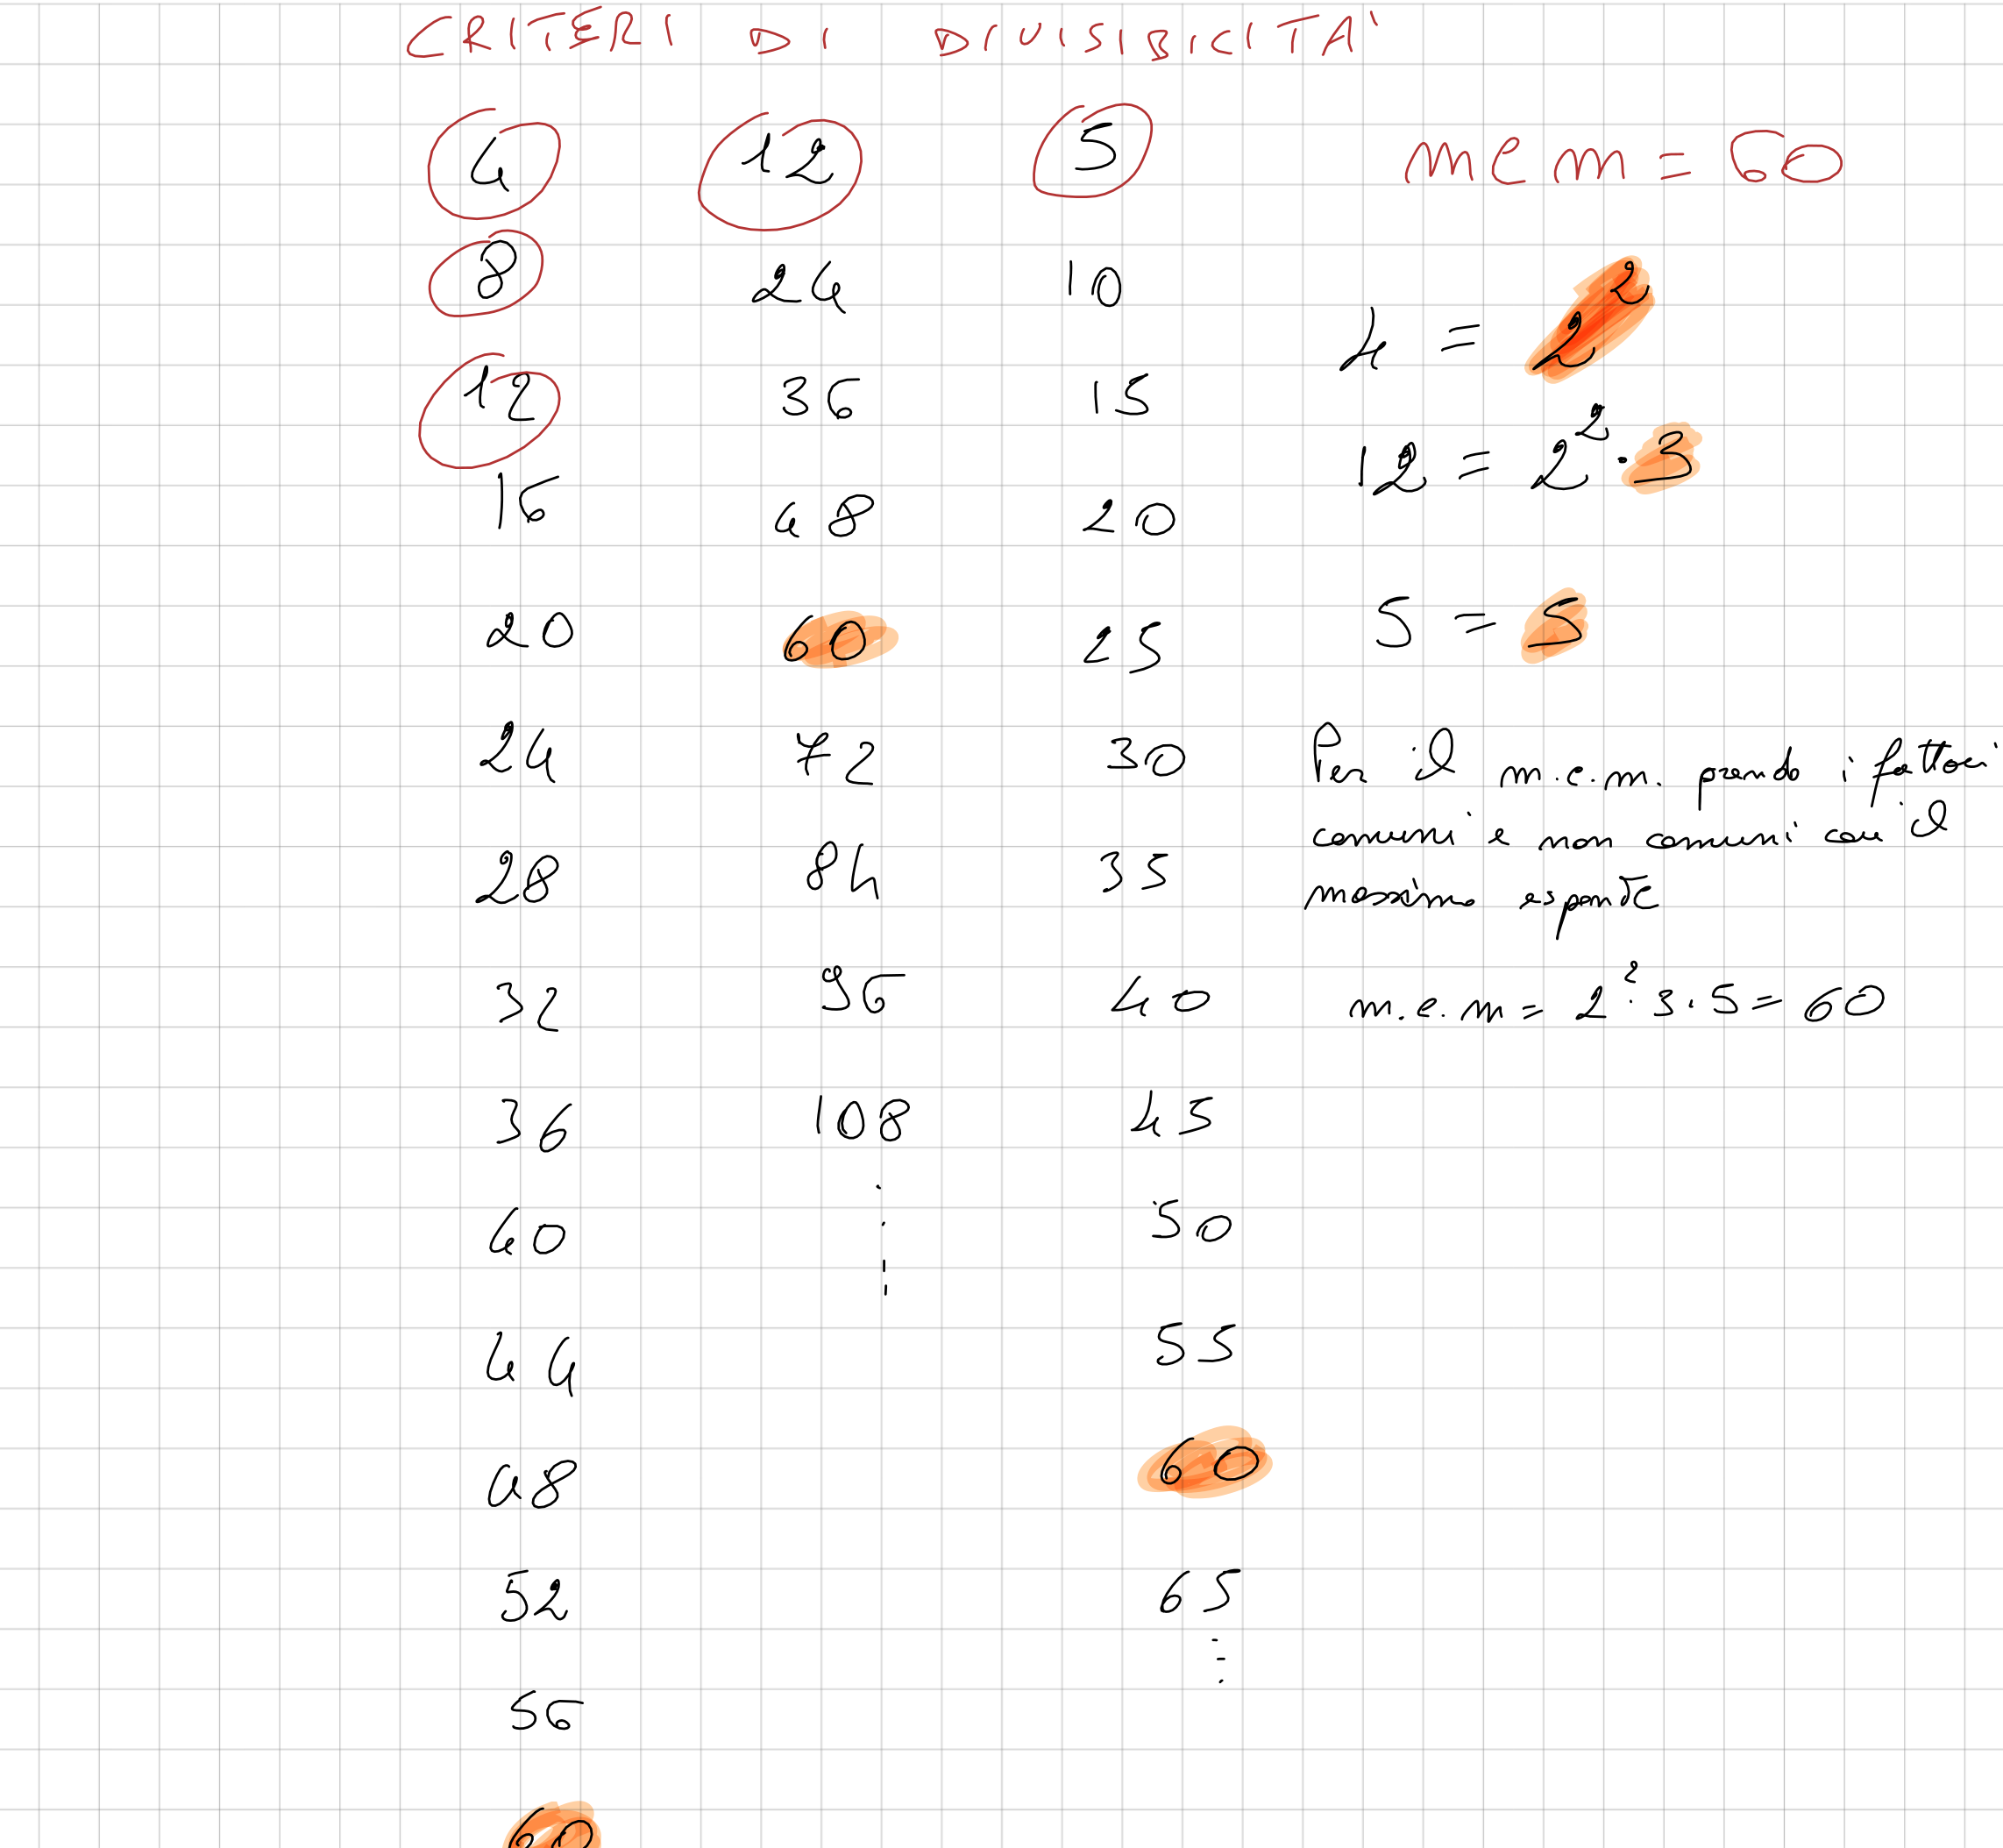
\includegraphics[width=0.88\linewidth]{immagini/appunti_tavola6_mcm.png}
\caption{Riproduzione fedele della Tavola 6 originale (Parte 1): calcolo tabulare per enumerazione di $\mathrm{mcm}(4, 12, 5) = 60$ e fattorizzazione analitica.}
\end{figure}

\begin{figure}[H]
\centering
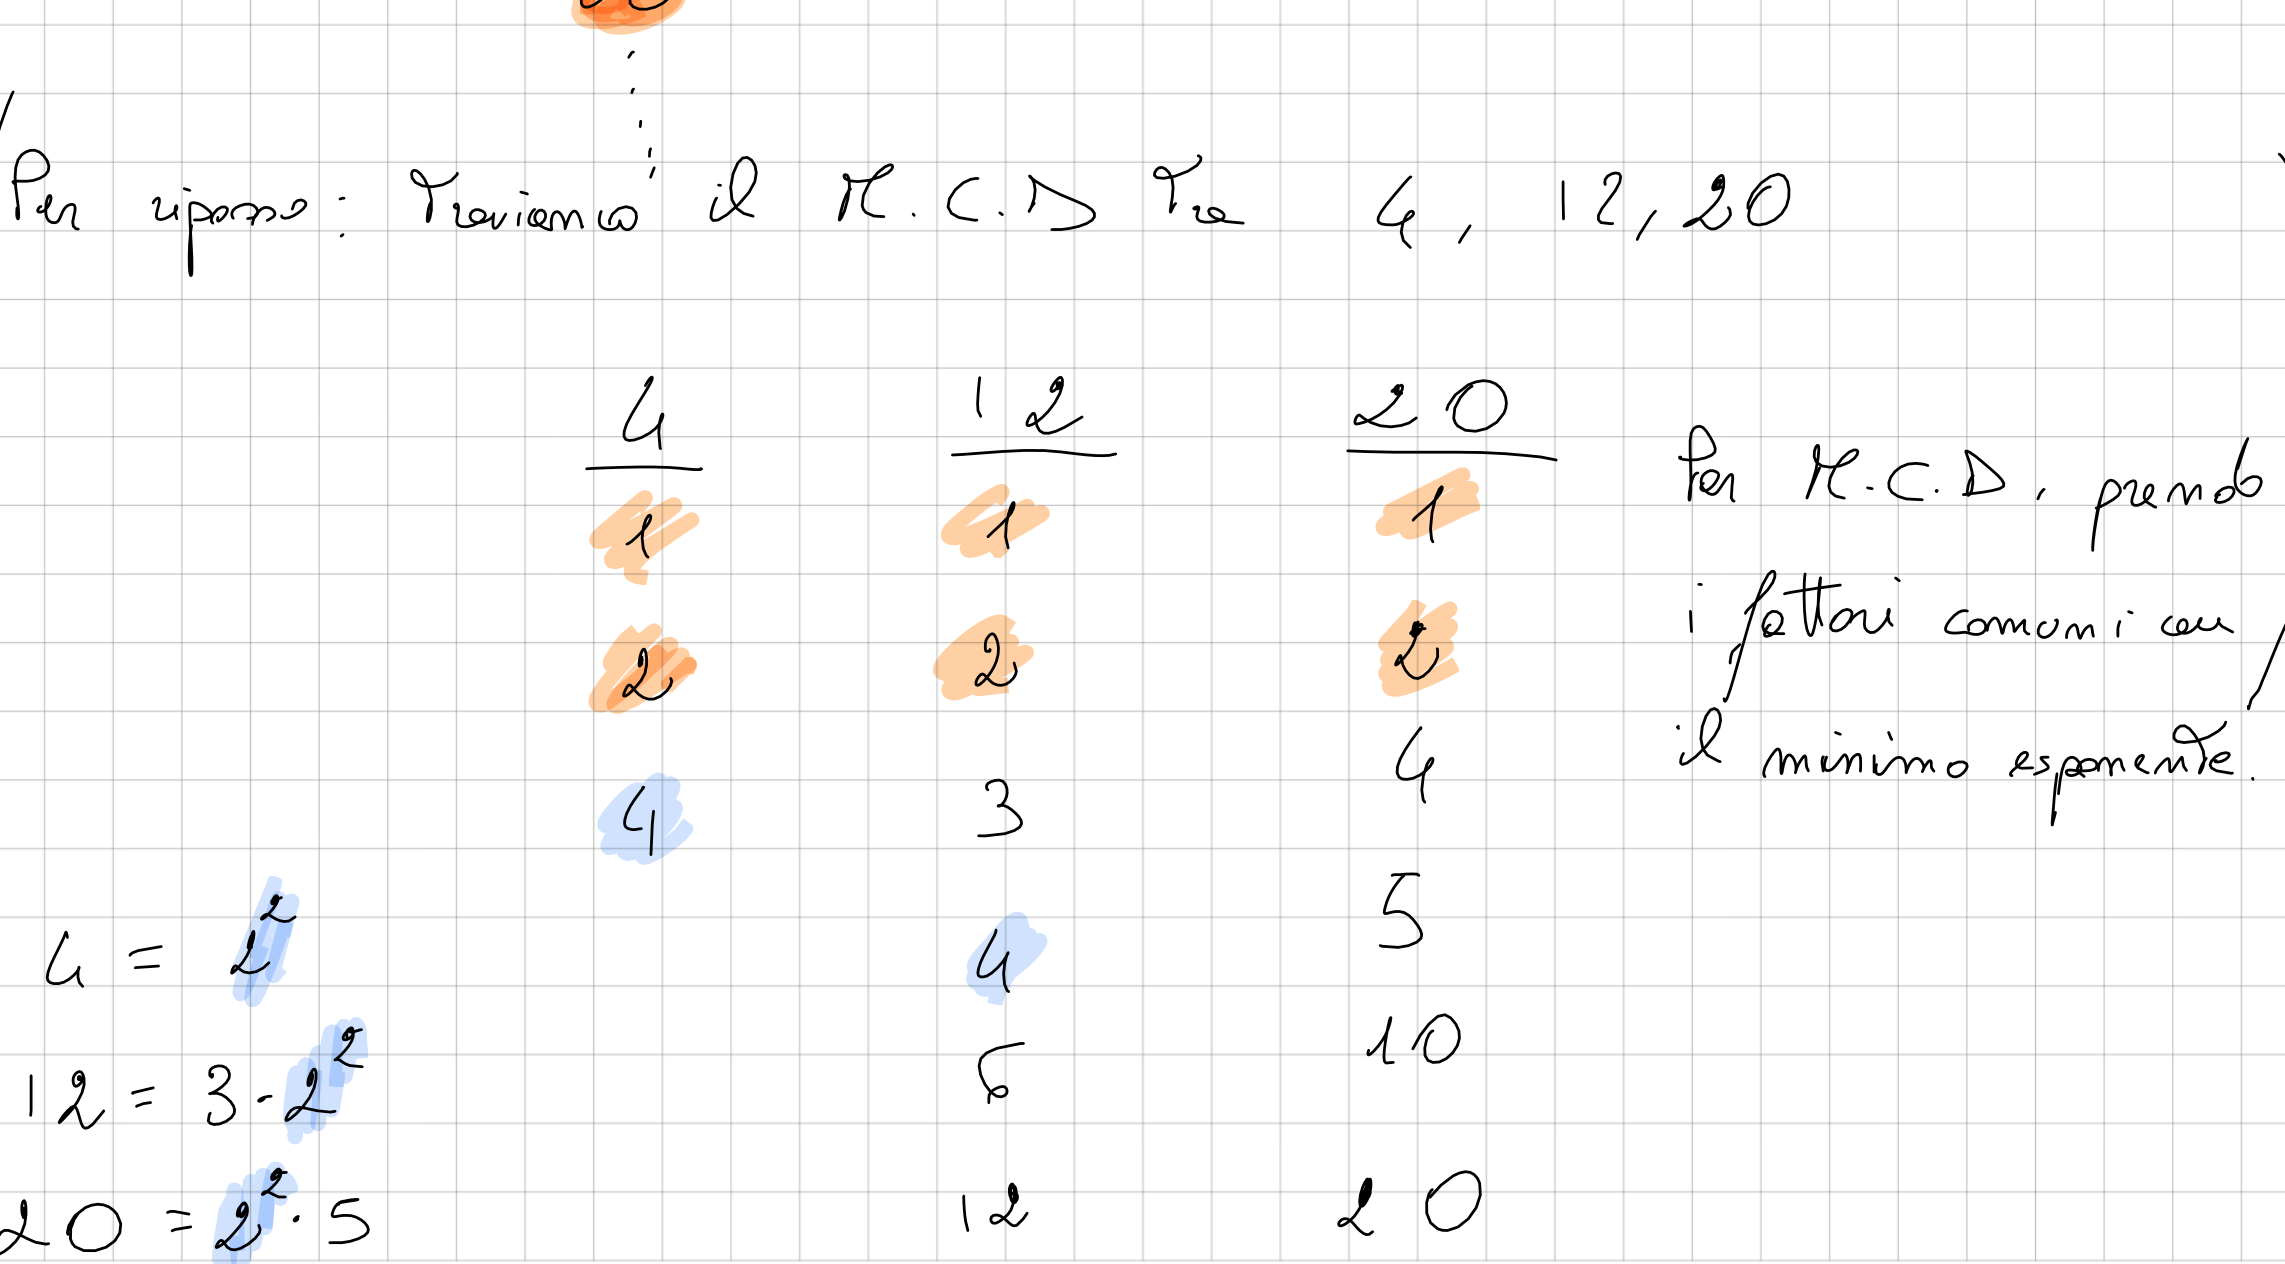
\includegraphics[width=0.88\linewidth]{immagini/appunti_tavola6_mcd.png}
\caption{Riproduzione fedele della Tavola 6 originale (Parte 2): calcolo tabulare per enumerazione dei divisori e determinazione di $\mathrm{MCD}(4, 12, 20) = 4$.}
\end{figure}

\begin{figure}[H]
\centering
\resizebox{0.96\linewidth}{!}{%
\begin{tikzpicture}[x=1cm, y=1cm]
  % Box mcm
  \draw[thick, primaryBlue, rounded corners=8pt, fill=blue!3!white] (-0.2, -8.0) rectangle (7.2, 1.1);
  \node[primaryBlue, font=\bfseries\sffamily] at (3.5, 0.6) {Determinazione di $\mathrm{mcm}(4, 12, 5) = 60$};
  
  \node[font=\bfseries, text=primaryBlue] at (1.1, -0.05) {$\mathcal{M}(4)$};
  \node[font=\bfseries, text=primaryBlue] at (3.5, -0.05) {$\mathcal{M}(12)$};
  \node[font=\bfseries, text=primaryBlue] at (5.9, -0.05) {$\mathcal{M}(5)$};
  \draw[gray!30] (0.1, -0.35) -- (6.9, -0.35);
  
  % Multipli di 4
  \foreach \val [count=\i] in {4,8,12,16,20,24,28,32,36,40,44,48,52,56} {
    \pgfmathsetmacro{\ypos}{-0.35 - \i*0.38}
    \node[font=\small, text=textDark] at (1.1, \ypos) {\val};
  }
  \node[font=\small\bfseries, text=accentAmber, fill=amber!20, inner sep=2pt, rounded corners=2pt] at (1.1, -6.05) {60};

  % Multipli di 12
  \foreach \val [count=\i] in {12,24,36,48} {
    \pgfmathsetmacro{\ypos}{-0.35 - \i*0.38}
    \node[font=\small, text=textDark] at (3.5, \ypos) {\val};
  }
  \node[font=\small\bfseries, text=accentAmber, fill=amber!20, inner sep=2pt, rounded corners=2pt] at (3.5, -2.25) {60};
  \node[font=\small, text=textDark] at (3.5, -2.63) {72};
  \node[font=\small, text=textDark] at (3.5, -3.01) {84};

  % Multipli di 5
  \foreach \val [count=\i] in {5,10,15,20,25,30,35,40,45,50,55} {
    \pgfmathsetmacro{\ypos}{-0.35 - \i*0.38}
    \node[font=\small, text=textDark] at (5.9, \ypos) {\val};
  }
  \node[font=\small\bfseries, text=accentAmber, fill=amber!20, inner sep=2pt, rounded corners=2pt] at (5.9, -4.91) {60};
  
  \draw[thick, accentAmber, fill=amber!15, rounded corners=4pt] (0.6, -7.60) rectangle (6.4, -6.95);
  \node[accentAmber!90!black, font=\small\bfseries] at (3.5, -7.275) {Minimo comune multiplo = 60};

  % Box MCD
  \begin{scope}[xshift=8.0cm]
    \draw[thick, accentGreen, rounded corners=8pt, fill=green!3!white] (-0.2, -8.0) rectangle (7.2, 1.1);
    \node[accentGreen!80!black, font=\bfseries\sffamily] at (3.5, 0.6) {Determinazione di $\mathrm{MCD}(4, 12, 20) = 4$};
    
    \node[font=\bfseries, text=accentGreen!80!black] at (1.1, -0.05) {$\mathcal{D}(4)$};
    \node[font=\bfseries, text=accentGreen!80!black] at (3.5, -0.05) {$\mathcal{D}(12)$};
    \node[font=\bfseries, text=accentGreen!80!black] at (5.9, -0.05) {$\mathcal{D}(20)$};
    \draw[gray!30] (0.1, -0.35) -- (6.9, -0.35);

    % Divisori di 4
    \node[font=\small\bfseries, text=primaryBlue] at (1.1, -0.73) {1};
    \node[font=\small\bfseries, text=primaryBlue] at (1.1, -1.11) {2};
    \node[font=\small\bfseries, text=accentRed, fill=red!20, inner sep=2pt, rounded corners=2pt] at (1.1, -1.49) {4};

    % Divisori di 12
    \node[font=\small\bfseries, text=primaryBlue] at (3.5, -0.73) {1};
    \node[font=\small\bfseries, text=primaryBlue] at (3.5, -1.11) {2};
    \node[font=\small, text=textDark] at (3.5, -1.49) {3};
    \node[font=\small\bfseries, text=accentRed, fill=red!20, inner sep=2pt, rounded corners=2pt] at (3.5, -1.87) {4};
    \node[font=\small, text=textDark] at (3.5, -2.25) {6};
    \node[font=\small, text=textDark] at (3.5, -2.63) {12};

    % Divisori di 20
    \node[font=\small\bfseries, text=primaryBlue] at (5.9, -0.73) {1};
    \node[font=\small\bfseries, text=primaryBlue] at (5.9, -1.11) {2};
    \node[font=\small\bfseries, text=accentRed, fill=red!20, inner sep=2pt, rounded corners=2pt] at (5.9, -1.49) {4};
    \node[font=\small, text=textDark] at (5.9, -1.87) {5};
    \node[font=\small, text=textDark] at (5.9, -2.25) {10};
    \node[font=\small, text=textDark] at (5.9, -2.63) {20};

    \draw[thick, accentRed, fill=red!15, rounded corners=4pt] (0.6, -7.60) rectangle (6.4, -6.95);
    \node[accentRed!90!black, font=\small\bfseries] at (3.5, -7.275) {Massimo comune divisore = 4};
  \end{scope}
\end{tikzpicture}%
}
\caption{Visualizzazione tabulare sinottica per la determinazione di $\mathrm{mcm}$ e $\mathrm{MCD}$ (conforme alla Tavola 6, a spaziatura verticale rigorosa anti-sovrapposizione).}
\end{figure}

% ==============================================================================
% CAPITOLO 4
% ==============================================================================
\chapter{L'Approssimazione Razionale del Numero \texorpdfstring{$\pi$}{pi}}

\section{Definizione Geometrica e Incommensurabilit\`a}
\begin{definizione}[Rapporto Circonferenza-Diametro]
In geometria euclidea, il rapporto tra la lunghezza della circonferenza $C$ e il suo diametro $d = 2r$ \`e una costante universale indipendente dalle dimensioni del cerchio, indicata con la lettera greca $\pi$:
\[
\pi = \frac{C}{d} = 3{,}141592653589793238\dots
\]
Come dimostrato da Johann Heinrich Lambert nel 1761, $\pi$ \`e un \textbf{numero irrazionale}: la circonferenza e il diametro sono grandezze tra loro \textbf{incommensurabili}, ossia non esiste alcuna unit\`a di misura comune sottomultipla che possa misurare esattamente entrambi con numeri interi.
Pertanto, $\pi$ non pu\`o essere espresso esattamente sotto forma di frazione $\frac{p}{q}$ ($p, q \in \mathbb{Z}$), n\'e possiede uno sviluppo decimale periodico.
\end{definizione}

\begin{figure}[H]
\centering
\begin{tikzpicture}[scale=0.85]
  % Circonferenza
  \draw[ultra thick, primaryBlue] (0, 1.6) circle (1.6cm);
  \coordinate (O) at (0, 1.6);
  \fill[primaryBlue] (O) circle (3pt) node[above right] {$O$};
  
  % Diametro d
  \draw[thick, accentRed, {Latex[length=2mm]}-{Latex[length=2mm]}] (-1.6, 1.6) -- (1.6, 1.6);
  \node[accentRed, above, font=\bfseries] at (0, 1.6) {$d = 2r$};

  % Srotolamento della circonferenza su asse rettilineo
  \draw[->, thick, gray!80] (-1.8, -0.6) -- (11.5, -0.6) node[right, black] {$x$};
  
  % Tacche unità
  \foreach \x in {0,1,2,3,4,5,6,7,8,9,10} {
    \draw[gray] (\x, -0.5) -- (\x, -0.7);
  }
  
  % Lunghezza srotolata C = pi * d
  \draw[ultra thick, primaryBlue] (0, -0.6) -- (9.4248, -0.6);
  \fill[primaryBlue] (0, -0.6) circle (3pt) node[below] {$0$};
  \fill[accentRed] (9.4248, -0.6) circle (3pt) node[below] {$C = \pi \cdot d \approx 3{,}1416 \cdot d$};

  \node[font=\small, align=center] at (5.0, 3.6) {
    $\dfrac{C}{d} = \pi \implies C = \pi \cdot d$\\[0.15cm]
    \textit{Incommensurabilit\`a geometrica: nessun segmento razionale misura contemporaneamente $C$ e $d$}
  };
\end{tikzpicture}
\caption{Rappresentazione geometrica del rapporto fondamentale $\pi = C/d$ e rettificazione della circonferenza.}
\end{figure}

\section{La Mnemonica Letteraria Italiana delle 19 Cifre}
\begin{aneddoto}[Filastrocca Mnemonica di Aritmetica Letteraria (Tavola 5 del Manoscritto)]
Per memorizzare con estrema facilit\`a le prime 19 cifre decimali di $\pi$, la tradizione scolastica italiana ha tramandato una celebre frase in cui il \textbf{numero di lettere di ciascuna parola corrisponde esattamente alla corrispondente cifra decimale}:
\begin{center}
{\large\textbf{«Ave o Roma o madre gagliarda di latine virt\`u,\\ che tanto luminoso splendore prodiga spargesti con la tua saggezza.»}}
\end{center}
Decodifichiamo analiticamente termine per termine la corrispondenza biunivoca:
\begin{center}
\small
\begin{tabular}{lccccccccc}
\toprule
\textbf{Parola} & Ave & o & Roma & o & madre & gagliarda & di & latine & virt\`u \\
\midrule
\textbf{Lettere} & \textbf{3} & \textbf{1} & \textbf{4} & \textbf{1} & \textbf{5} & \textbf{9} & \textbf{2} & \textbf{6} & \textbf{5} \\
\midrule
\midrule
\textbf{Parola} & che & tanto & luminoso & splendore & prodiga & spargesti & con & la & tua \\
\midrule
\textbf{Lettere} & \textbf{3} & \textbf{5} & \textbf{8} & \textbf{9} & \textbf{7} & \textbf{9} & \textbf{3} & \textbf{2} & \textbf{3} \\
\bottomrule
\end{tabular}
\end{center}
Completando con l'ultima parola \textbf{saggezza} ($8$ lettere), si ottiene la sequenza esatta:
\[
\pi \approx \mathbf{3{,}141592653589793238}
\]
\end{aneddoto}

\section{Cronologia e Confronto delle Frazioni Razionali Approssimanti}
\begin{metodo}[Analisi Comparativa dell'Errore Relativo (Tavola 5 del Manoscritto)]
Poich\'e $\pi$ \`e irrazionale, l'ingegneria, l'astronomia e l'architettura storica hanno fatto ricorso a frazioni razionali $\frac{p}{q}$ aventi denominatori piccoli e precisione massimizzata:
\begin{itemize}[leftmargin=2em]
  \item \textbf{Approssimazione Babilonese (XVIII sec. a.C.):} $\dfrac{25}{8} = 3{,}125000$. Ottenuta assimilando il perimetro dell'esagono inscritto alla circonferenza con un correttivo di $\frac{1}{8}$.
  \item \textbf{Approssimazione Egizia (Papiro di Rhind, XVII sec. a.C.):} $\left(\dfrac{16}{9}\right)^2 = \dfrac{256}{81} \approx 3{,}160494$. Derivata dalla quadratura empirica del cerchio inscritto in un quadrato di lato 9.
  \item \textbf{Approssimazione di Archimede (Siracusa, III sec. a.C.):} $\dfrac{22}{7} \approx 3{,}142857$. Calcolata mediante il metodo dei poligoni regolari inscritti e circoscritti di $96$ lati: $\frac{223}{71} < \pi < \frac{22}{7}$.
  \item \textbf{Approssimazione di Zu Chongzhi (Cina, V sec. d.C.):} $\dfrac{355}{113} \approx 3{,}14159292$. Conosciuta come \textit{Mil\"u}, fornisce un accordo prodigioso esatto fino alla sesta cifra decimale.
\end{itemize}
\end{metodo}

\begin{table}[H]
\centering
\small
\renewcommand{\arraystretch}{1.25}
\begin{tabularx}{\textwidth}{>{\raggedright\arraybackslash}X c c c r}
\toprule
\textbf{Civilt\`a / Matematico} & \textbf{Frazione $\frac{p}{q}$} & \textbf{Valore Decimale} & \textbf{Errore Assoluto} & \textbf{Errore \%} \\
\midrule
Antica Babilonia & $\dfrac{25}{8}$ & $3{,}125000\dots$ & $-1{,}66 \cdot 10^{-2}$ & $-0{,}53\%$ \\
\addlinespace
Antico Egitto (Rhind) & $\dfrac{256}{81}$ & $3{,}160494\dots$ & $+1{,}89 \cdot 10^{-2}$ & $+0{,}60\%$ \\
\addlinespace
Archimede di Siracusa & $\dfrac{22}{7}$ & $3{,}142857\dots$ & $+1{,}26 \cdot 10^{-3}$ & $+0{,}04\%$ \\
\addlinespace
Zu Chongzhi (Mil\"u) & $\dfrac{355}{113}$ & $3{,}14159292\dots$ & $+2{,}67 \cdot 10^{-7}$ & $+0{,}0000085\%$ \\
\addlinespace
\midrule
\textbf{Valore Reale Esatto} & $\bm{\pi}$ & $\mathbf{3{,}14159265\dots}$ & $\mathbf{0}$ & \textbf{Esatto} \\
\bottomrule
\end{tabularx}
\caption{Confronto analitico delle principali frazioni approssimanti razionali di $\pi$.}
\end{table}

% ==============================================================================
% SEZIONI INTEGRATIVE: FRAZIONI CONTINUE DI PI GRECO E RADICE DI 2 (TAVOLE 5 E 6)
% ==============================================================================
\section{Lo Sviluppo in Frazione Continua di \texorpdfstring{$\pi$}{pi} e la Frazione di Zu Chongzhi (Tavola 5)}

\begin{definizione}[Frazione Continua Semplice]
Una \textbf{frazione continua semplice} \`e un'espressione matematica della forma:
\begin{equation}
    x = a_0 + \cfrac{1}{a_1 + \cfrac{1}{a_2 + \cfrac{1}{a_3 + \dots}}}
\end{equation}
dove $a_0 \in \mathbb{Z}$ e $a_1, a_2, a_3, \dots$ sono interi positivi ($a_i \ge 1$), detti \textbf{quozienti parziali}. Troncare la frazione a un determinato livello produce una frazione razionale $\frac{p_k}{q_k}$, detta \textbf{convergente}, che costituisce la \textbf{migliore approssimazione razionale possibile} di $x$ rispetto a qualsiasi altra frazione avente denominatore non superiore a $q_k$.
\end{definizione}

\begin{laboratorio}[Sviluppo Algoritmico della Frazione Continua di $\pi$ (Tavola 5)]
Come evidenziato negli appunti della Tavola 5, per il numero $\pi$ si ha:
\begin{equation}
    \pi = 3 + \cfrac{1}{7 + \cfrac{1}{16 + \dots}}
\end{equation}
Calcoliamo esplicitamente le convergenti razionali intermedie:
\begin{enumerate}[leftmargin=2em]
    \item \textbf{Troncamento al livello intermedio con denominatore 15:}
    \begin{equation}
    \begin{aligned}
        3 + \cfrac{1}{7 + \dfrac{1}{15}} &= 3 + \cfrac{1}{\dfrac{105 + 1}{15}} = 3 + \frac{15}{106} \\
        &= \frac{3 \cdot 106 + 15}{106} = \mathbf{\frac{333}{106}} \approx \mathbf{3{,}1415094\dots}
    \end{aligned}
    \end{equation}
    
    \item \textbf{Troncamento al quoziente autentico 16 (Frazione di Zu Chongzhi):}
    \begin{equation}
    \begin{aligned}
        3 + \cfrac{1}{7 + \dfrac{1}{16}} &= 3 + \cfrac{1}{\dfrac{112 + 1}{16}} = 3 + \frac{16}{113} \\
        &= \frac{3 \cdot 113 + 16}{113} = \mathbf{\boxed{\frac{355}{113}}}
    \end{aligned}
    \end{equation}
    Il valore numerico di $\frac{355}{113}$ \`e:
    \begin{equation}
        \frac{355}{113} \approx \mathbf{3{,}14159292\dots}
    \end{equation}
    Confrontato con il valore reale $\pi = \mathbf{3{,}14159265\dots}$, l'errore \`e di appena $2{,}7 \cdot 10^{-7}$! Questa frazione garantisce ben sei cifre decimali esatte con un denominatore di appena tre cifre.
\end{enumerate}
\end{laboratorio}

\section{Lo Sviluppo in Frazione Continua di \texorpdfstring{$\sqrt{2}$}{sqrt(2)} e la Periodicit\`a (Tavole 5 e 6)}

\begin{laboratorio}[Algoritmo di Sviluppo per $\sqrt{2}$ dalle Tavole 5 e 6 del Docente]
Consideriamo il numero irrazionale quadratico:
\begin{equation}
    \sqrt{2} = 1{,}41421356237\dots
\end{equation}
Isoliamo la parte intera e la parte decimale:
\begin{equation}
    \sqrt{2} = 1 + (\sqrt{2} - 1) = 1 + 0{,}4142135\dots
\end{equation}
Invertiamo la parte decimale:
\begin{equation}
    \frac{1}{0{,}4142135\dots} = \frac{1}{\sqrt{2} - 1} = \frac{\sqrt{2} + 1}{(\sqrt{2} - 1)(\sqrt{2} + 1)} = \sqrt{2} + 1 = 2{,}4142135\dots
\end{equation}
Procediamo iterativamente per ricavare i successivi convergenti razionali:
\begin{itemize}[leftmargin=2em]
    \item \textbf{$1^\circ$ Ordine:} $\sqrt{2} \approx \mathbf{1}$
    \item \textbf{$2^\circ$ Ordine:} $\sqrt{2} = 1 + \cfrac{1}{2{,}414\dots} \approx 1 + \frac{1}{2} = \mathbf{1{,}5} = \mathbf{\frac{3}{2}}$
    \item \textbf{$3^\circ$ Ordine (Tavola 6):}
    \begin{equation}
        \sqrt{2} = 1 + \cfrac{1}{2 + \dfrac{1}{2{,}414\dots}} \approx 1 + \cfrac{1}{2 + \dfrac{1}{2}} = 1 + \cfrac{1}{\dfrac{5}{2}} = 1 + \frac{2}{5} = \frac{5 + 2}{5} = \mathbf{\boxed{\frac{7}{5}}} = \mathbf{1{,}4}
    \end{equation}
\end{itemize}
\end{laboratorio}

\begin{metodo}[La Frazione Continua Periodica Infinita di $\sqrt{2}$]
Poich\'e ad ogni passo di inversione la parte decimale residua si ripete identicamente ($2{,}4142135\dots - 2 = 0{,}4142135\dots$), il quoziente parziale \`e perennemente pari a $2$.
La frazione continua di $\sqrt{2}$ \`e quindi \textbf{periodica infinita}:
\begin{equation}
    \mathbf{\sqrt{2} = 1 + \cfrac{1}{2 + \cfrac{1}{2 + \cfrac{1}{2 + \cfrac{1}{2 + \dots}}}}} = \bm{[1; \, \overline{2}]}
\end{equation}
\textbf{Dimostrazione Algebrica Elegante:}\\
Posto $x = \sqrt{2} - 1$, si ha:
\begin{align}
    x + 1 = \sqrt{2} &\implies (x + 1)^2 = 2 \implies x^2 + 2x + 1 = 2 \\
    &\implies x^2 + 2x = 1 \implies x(x + 2) = 1 \implies x = \frac{1}{2 + x}
\end{align}
Sostituendo iterativamente l'espressione $x = \frac{1}{2 + x}$ dentro se stessa:
\begin{equation}
    x = \cfrac{1}{2 + \cfrac{1}{2 + \cfrac{1}{2 + \dots}}} \implies \sqrt{2} = 1 + x = 1 + \cfrac{1}{2 + \cfrac{1}{2 + \cfrac{1}{2 + \dots}}} \qedhere
\end{equation}
\end{metodo}

\end{document}
